%------------------
%	PRZEWODNIK PO UBUNTU 14.04 LTS TRUSTY THAR
%	
%
%	Autorzy:
%		1. Piotr "Dwimenor Vali" Sochocki, dwimeron@gmail.com
%
%	Licencja:
%		Creative Commons
%		Uznanie autorstwa-Uzycie niekomercyjne-Na tych samych warunkach 3.0 Polska
%		CC BY-NC-SA 3.0 PL
%		http://creativecommons.org/licenses/by-nc-sa/3.0/pl/
%------------------


%------------------
%	PREAMBUŁA
%------------------
%TODO użyj paczki menukeys wszędzie tam, gdzie każe się coś wcisnąć na klawiaturze.

% klasa mwart autorstwa Marcina Wolińskiego
% http://marcinwolinski.pl/mwcls.html
% pakiet: texlive-lang-polish
\documentclass[a4paper,11pt,oneside]{mwart}

% orientacja pozioma, marginesy
\usepackage[landscape, margin=0.5in]{geometry}

% interlinia (1.6 = półtora linni odstępu wg. nomenklatury Worda/Writera)
\linespread{1.6}

% Odległosć między akapitami
\setlength{\parskip}{0.2cm}

% Język polski, polfonty
\usepackage[OT4]{polski}
\usepackage[utf8]{inputenc}

% dzielenie wierszy
\brokenpenalty=1000
\clubpenalty=1000
\widowpenalty=1000

% Obrazki
\usepackage{graphicx}
\usepackage{wrapfig}

% linki, URL
\usepackage[urlcolor=blue, colorlinks=true]{hyperref} 

% Dwie kolumny w spisie treści
\usepackage[toc]{multitoc}

% Jako, że nie bawimy się w rozdziały, sekcja i podsekcja są podstawowymi jednostmaki podziału dokumentu.
% Poniższa komenda wymusza numerowanie sekcji od "1" zamiast od "0"
\renewcommand*\thesection{\arabic{section}}

% Gwizadka zamiast myślnika jak znak kolejnego punktu listy.
\renewcommand{\labelitemi}{$\star$}

% Oficjalne kolory Ubuntu
% http://design.ubuntu.com/brand/colour-palette
\usepackage{xcolor}
\definecolor{ubuntu_orange}{RGB}{221,72,20}

%------------------
%	STRUKTURA DOKUMENTU
%------------------

\begin{document}

\thispagestyle{empty}

%-----------------
%	TYTUŁ
%-----------------

\colorbox{ubuntu_orange}{
	\parbox[t]{1.0\linewidth}{
		\centering \fontsize{40pt}{70pt}\selectfont
		\vspace*{0.7cm}
		
		\hfill Przewodnik po\\
		\hfill Ubuntu 14.04 LTS\\
		\hfill Trusty Thar\par
		
		\vspace*{0.7cm}
	}
}

\vfill

%-----------------
%	AUTOR
%-----------------

{
	\centering
	\large 
	\hfill Zespół \href{http://www.ubuntu.pl}{Ubuntu.pl} \\
}
\clearpage

\tableofcontents
\clearpage
\section{Wstęp}
	\noindent Witaj w \textcolor{ubuntu_orange}{Przewodniku po Ubuntu Linux 14.04 Trusty Thar!}

Niniejszy dokument pomoże ci zainstalować oraz skonfigurować system operacyjny Ubuntu. Przewodnik obejmuje każdy etap procesu zmiany systemu, od przygotowania twoich plików i ustawień po instalowanie oraz używanie twojej świeżo zainstalowanej kopii Ubuntu.

Przewodnik ten został napisany z myślą o osobach nieposiadających wiedzy technicznej, a większość terminów technicznych opatrzono stosownymi objaśnieniami. Przewodnik zadaje także kłam mitowi, że użytkowanie Linuksa wiąże się z koniecznością wpisywania niezrozumiałych komend w konsoli. Cały tekst został przygotowany z myślą o wykorzystaniu graficznych narzędzi dostarczanych wraz z systemem.

Mamy nadzieję, że czytając ten przewodnik bezproblemowo zainstalujesz Ubuntu na swoim komputerze i będziesz zadowolony mogąc korzystać z darmowego oraz otwartego systemu operacyjnego.\\
Wersja Ubuntu, która została opisana w tym poradniku, nosi nazwę Ubuntu GNU/Linux 14.04 LTS Trusty Thar, co oznacza:
\begin{itemize}
\item \textcolor{ubuntu_orange}{Ubuntu} ---  nazwa całej serii systemów operacyjnych wydawanych przez firmę Canonical.
\item \textcolor{ubuntu_orange}{GNU/Linux} --- system bazuje na jądrze Linuksa i wykorzystuje oprogramowanie GNU.
\item \textcolor{ubuntu_orange}{14.04} --- jest to wersja z kwietnia (04) 2014 roku.
\item \textcolor{ubuntu_orange}{LTS} --- jest to wersja o przedłużonym wsparciu technicznym, a poprawki będą wydawane do 2019 roku).
\item \textcolor{ubuntu_orange}{Trusty Tahr} --- nazwa kodowa tego wydania.
\end{itemize}
	\subsection{O Ubuntu}
		Ubuntu jest kompletnym systemem operacyjnym utrzymywanym i rozwijanym przez firmę Canonical. Pierwsza jego wersja ukazała się w 2004 roku, a w ciągu14 lat system ten zdobył rzesze fanów. Ubuntu wraz ze swoimi odmianami jest najpopularniejszą na świecie dystrybucją Linuksa. Samo słowo Ubuntu w języku afrykańskiego plemienia Zulusów oznacza ”człowieczeństwo wobec innych”, w kontekście systemu operacyjnego tłumaczone jest jednak jako ”Linux dla ludzi”.

Ideą systemu Ubuntu jest dostarczenie użytkownikowi kompletnego systemu operacyjnego, zawierającego wszystkie elementy niezbędne do codziennej pracy, a jednocześnie umożliwiające posiadaczowi komputera swobodne korzystanie z systemu i modyfikowanie poszczególnych jego elementów. Wybierając Ubuntu nie musisz się zastanawiać nad tym, czy twój procesor nie ma przypadkiem zbyt dużej liczby rdzeni, co w przypadku korzystania z systemu komercyjnego mogłoby wymagać zakupu innej licencji. Nie musisz się również przejmować tym, że w firmie masz dziesięć komputerów, a twoja licencja na pakiet biurowy pozwala na instalację jedynie na sześciu stanowiskach. Jeśli chodzi o to, jak i do czego wykorzystasz system i oprogramowanie, wszystko zależy wyłącznie od ciebie.

Ubuntu pozwala także na daleko idące modyfikacje systemu - kod źródłowy jest otwarty, co pozwala każdemu na głębokie ingerencje w system. Choć powyższe zdanie może brzmieć groźnie, nie ma powodów do obaw - Ubuntu nie jest przeznaczone tylko dla doświadczonych komputerowych “magików”. Każdy może dowolnie dostosować swój system do własnych potrzeb i upodobań, czy to metodą zrób to sam, czy też poprzez odwołanie się do zasobów oferowanych przez społeczność.

Skoro poruszyliśmy już ten temat - społeczność skupiona wokół Ubuntu jest najważniejszą siłą napędzającą rozwój tej dystrybucji. Dodatki zmieniające wygląd systemu, nowe ikony i grafiki, dźwięki systemowe, tłumaczenia, całe zestawy oprogramowania - wszystkie te elementy (oraz wiele innych rzeczy) czekają, aż zdecydujesz się z nich skorzystać.
\clearpage

	\subsection{Dlaczego warto zmienić system na Ubuntu?}
		\subsubsection{Jest stabilny}
Ubuntu bazuje na słynącym ze stabilności systemie Debian GNU/Linux. Zapomnij o błędach krytycznych i zawieszaniu się komputera, przyzwyczaj się natomiast do niezawodnego systemu, który po prostu działa. Standardy jakości Debiana są bardzo wysokie i do ostatecznej wersji tego systemu nie trafi nic, co mogłoby nagle się popsuć. Jeśli instalujesz pod Ubuntu jakąś aplikację, możesz mieć pewność, że została już ona przetestowana przez tysiące ludzi rozsianych po całym świecie.
\begin{itemize}
\item Debian GNU/Linux jest tak stabilny, że pod jego kontrolą pracują najważniejsze systemy komputerowe świata, wliczając w to superkomputery oraz serwery wielkich portali internetowych.
\item Poprawki eliminujące znalezione błędy trafiają do systemu na bieżąco i nie trzeba na nie czekać miesiącami.
\item Każdy może zgłaszać znalezione błędy i śledzić proces ich naprawiania.
\end{itemize}
\subsubsection{Jest bezpieczny}
Ubuntu prezentuje zupełnie inne podejście do zagadnienia bezpieczeństwa niż inne systemy operacyjne. Tutaj bezpieczeństwo wynika z samej konstrukcji systemu,nie jest natomiast rezultatem nakładania na niego kolejnych łatek i dodatkowych warstw ochronnych. System jest bezpieczny, ponieważ likwiduje się przyczynę ewentualnych problemów, a nie leczy objawy. Co więcej, błędy, które mogłyby mieć negatywny wpływ na bezpieczeństwo użytkownika, naprawiane są niemal natychmiast. Nierzadko zdarza się, że od momentu wykrycia luki do chwili instalacji stosownej poprawki na milionach komputerów mija mniej niż doba.
\begin{itemize}
\item Ponieważ różne dystrybucje Linuksa cechują się wysokim poziomem bezpieczeństwa, to właśnie te systemy operacyjne można znaleźć na bardzo wielu serwerach sieciowych.
\item Wprowadzanie poważniejszych zmian w systemie pociąga za sobą konieczność podania hasła administratora. Ubuntu jest dzięki temu zabezpieczone zarówno przed potencjalnymi intruzami, jak i przed przypadkowym naruszeniem zasad bezpieczeństwa przez samego użytkownika.
\end{itemize}
\subsubsection{Jest łatwy w użyciu}
Słowo Ubuntu tłumaczy się jako ”\textit{człowieczeństwo wobec innych}”,  także “Linux dla ludzi”. Użytkowane przez ciebie programy zostały zaprojektowane w taki sposób, by nie były bardziej skomplikowane, niż to konieczne. To wcale nie znaczy, że Ubuntu ma ograniczone możliwości czy brakuje mocy - wręcz przeciwnie, pulpit Ubuntu jest pełen innowacyjnych funkcji.
\begin{itemize}
\item Komunikaty są sformułowane w jednoznaczny sposób, więc będziesz potrzebował przeczytać je tylko raz.
\item Aplikacje są ułożone tak, aby było je łatwo znaleźć.
\item Programy mają schludny i nowoczesny interfejs, dzięki któremu łatwiej będzie ci skupić się na czekających cię zadaniach.
\end{itemize}
\subsubsection{Jest międzynarodowy}
Nieważne gdzie mieszkasz i w jakim języku mówisz - możesz być pewien, że Ubuntu będzie się komunikowało z każdym użytkownikiem w najbardziej zrozumiały dla niego sposób. Dostęp do różnych wersji językowych jest bardzo prosty, a zmiana języka systemu ogranicza się do kilku kliknięć.
Oprócz  tłumaczeń obejmujących między innymi komunikaty systemowe, interfejs użytkownika czy menu poszczególnych aplikacji, Ubuntu oferuje również pełny wybór zestawów znaków i metod wprowadzania tekstu, możesz więc porozumiewać się ze swoim komputerem w dowolnie wybranym języku.
\begin{itemize}
\item Tłumaczenia są tworzone przez ochotników z całego świata.
\item Możesz samemu zaangażować się w tłumaczenia, korzystając z internetowej usługi Launchpad.
\item Aplikacja “Języki” pozwala szybko i wygodnie instalować nowe paczki językowe .
\end{itemize}
\subsubsection{Jest dostępny}
Świeżo zainstalowane Ubuntu wyposażone jest w szereg narzędzi poprawiających łatwość dostępu - lupę, program czytający informacje pojawiające się na ekranie oraz klawiaturę ekranową. Projekt Ubuntu posiada Zespół Dostępności, który zajmuje się wyłącznie tym, aby Ubuntu stawało się coraz bardziej dostępne dla każdego.
\begin{itemize}
\item Użytkownik może korzystać z ułatwień dostępu przez cały czas - od procesu instalacji począwszy, na codziennym użytkowaniu skończywszy.
\end{itemize}
\subsubsection{Jest wolny}
Ubuntu jest wolne i otwarte. Za instalację i użytkowanie tego systemu operacyjnego nigdy nie będziesz musiał zapłacić ani grosza. Nikt nie zabroni Ci również  modyfikowania, używania i rozprowadzania aplikacji wchodzących w skład Ubuntu. Nie musisz się zastanawiać nad tym, czy możesz wykorzystywać dany program, czy też jego licencja pozwala na przykład jedynie na ściśle określone zastosowania. W przypadku korzystania z Ubuntu nie ma takich ograniczeń - dysponujesz całkowitą wolnością w kwestii wykorzystywania i modyfikowania systemu oraz zawartego w nim oprogramowania.
Co więcej, zachęcamy cię do takiego postępowania! To oznacza, że zaoszczędzisz na oprogramowaniu, ale to nie wszystko - pamiętaj także, że jest ono całkowicie transparentne i otwarte na analizę. To pozwala szybciej wykrywać problemy związane z bezpieczeństwem, uniemożliwia ukrywanie przed niczego nieświadomym użytkownikiem przykrych niespodzianek, a na dodatek masz możliwość samodzielnego  dokonywania zmian w Ubuntu.
\begin{itemize}
\item Jeśli tylko posiadasz odpowiednią wiedzę techniczną, możesz samemu modyfikować swoje ulubione aplikacje.
\item Ubuntu może używać absolutnie każdy.
\end{itemize}
\subsubsection{Jest społecznościowy}
Społeczność to opoka, na której opiera się Ubuntu. Bez owej społeczności Ubuntu nie byłoby światowej klasy systemem operacyjnym, jakim jest w 2014 roku. Społeczność jest nierozłącznie związana z sukcesem Ubuntu i to właśnie ona zajmuje się wieloma rzeczami, od dostarczania tłumaczeń, testowania nowych wydań i zapewniani wsparcia, aż po pisanie nowego oprogramowania i rozwiązywanie problemów,  Każdy może pomóc w takim zakresie, w jakim potrafi i ma ochotę. Również i ty możesz pomóc kształtować kierunek rozwoju Ubuntu i ulepszać oprogramowanie dla ludzi z całego świata.
\begin{itemize}
\item Każdy może wnieść swój wkład w rozwój Ubuntu.
\item Ubuntu skupia ludzi posiadających bardzo różne zainteresowania. Programiści nie są jedynymi wybrańcami, którzy mają szansę zobaczyć efekty swojej pracy na milionach komputerów. Takie same możliwości mają graficy tworzacy tapety, muzycy komponujący dźwięki systemowe, designerzy projektujący ikony i zajmujący się wyglądem aplikacji, tłumacze dbający o to, by Ubuntu było dostępne w tylu językach, a także wiele, wiele innych osób.
\item Kodeks Postępowania Ubuntu i Rada Społeczności pomaga przewodzić społeczności i zapewnia każdemu możliwość przedstawienia swoich racji.
\end{itemize}
\clearpage

\section{Instalacja}
	\subsection{Pobieranie obrazu systemu}
		%TODO zweryfikować ten dokument jak już zaktualizują ubuntu.com
%obrazek
%linki
%rozmiar obrazów instalacyjnych
\begin{center}
	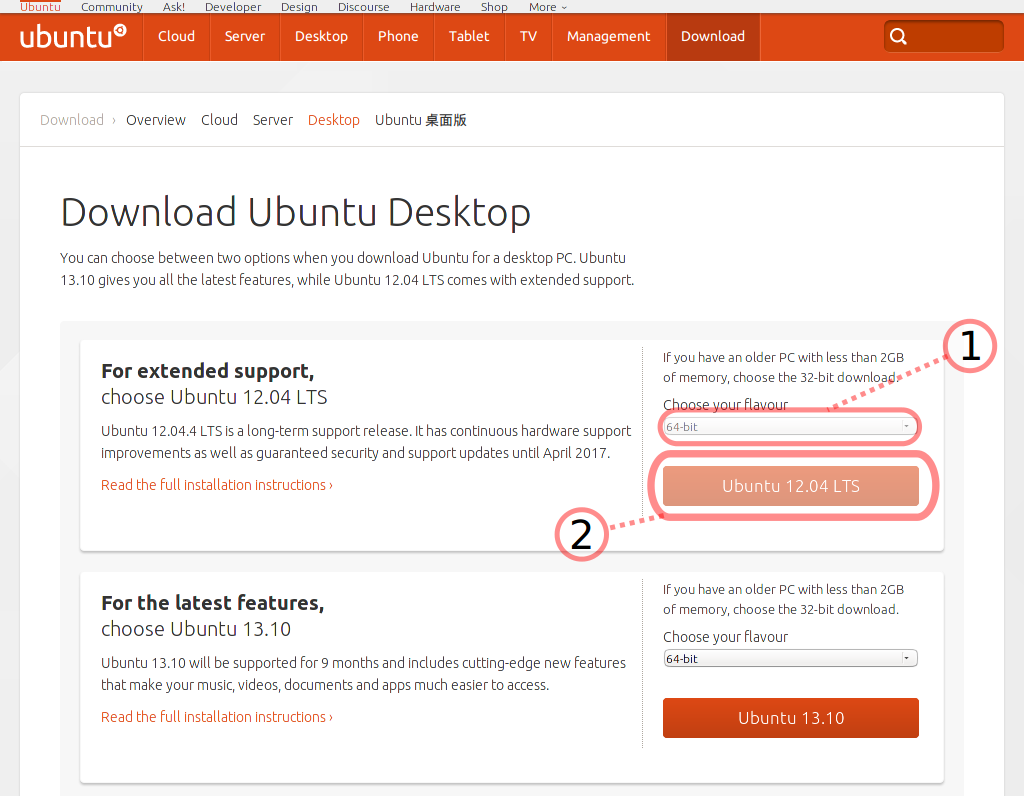
\includegraphics[width=\linewidth]{images/instalacja_pobieranie_obrazu.png}
\end{center}

Pierwszym etapem instalacji systemu jest pobranie instalatora. W tym celu udaj się na stronę \href{http://www.ubuntu.com/download/desktop}{ubuntu.com} i z górnego paska wybierz \textcolor{ubuntu_orange}{Download} a następnie \textcolor{ubuntu_orange}{Desktop}
\begin{enumerate}[label=\protect\circled{\arabic*}]
\item To pole pozwali ci wybrać pomiędzy 32- a 64-bitową wersją systemu. Domyślnie wybrana jest opcja 64 bitowa.
\item Kliknij na ten przycisk aby przejść dalej.
\end{enumerate}

Na kolejnym ekranie będziesz mieć możliwość przekazania dotacji na rzecz Ubuntu. W tym momencie nas to nie interesuje. Przesuń stronę w dół i kliknij na \textcolor{ubuntu_orange}{Not now, take me to the download}. Zostaniesz przeniesiony na kolejną stronę, a po kilku sekundach rozpocznie się pobieranie obrazu systemu.

Jeżeli twój komputer został wyprodukowany nie dawnej niż 5 lat temu, wersja 64-bitowa będzie na pewno odpowiednia. Jeżeli masz mniej niż 2 GB RAM-u, wybierz wariant 32-bitowy. Niezależnie od tego jaką wersję wybierzesz, i tak będziesz mieć dostęp do takiego samego zestawu oprogramowania. Wariant 64-bitowy jest lepiej dopasowany do nowoczesnych systemów, jeżeli jednak masz jakiekolwiek wątpliwości, wybierz wersję 32-bitową. Będzie ona działać także na 64-bitowym komputerze, choć nie będzie wykorzystywać wszystkich jego możliwości.
Jeżeli twoja płyta główna kontrolowana jest przez UEFI, musisz wybrać system 64-bitowy.
Linki do pobierania bezpośredniego:
\begin{itemize}
\item \href{http://www.ubuntu.com/start-download?distro=desktop&bits=64&release=lts}{Wersja 64 bitowa (733 megabajtów).}
\item \href{http://www.ubuntu.com/start-download?distro=desktop&bits=32&release=lts}{Wersja 32 bitowa (731 megabajtów).}
\end{itemize}
	\subsection{Nagrywanie pobranego obrazu}
		Po zakończeniu pobierania obrazu instalatora należy nagrać go na zewnętrzny nośnik i uruchomić komputer z tego nośnika. Najlepszym rozwiązaniem jest użycie klucza usb (pendriva), gdyż obrazy instalacyjne Ubuntu są zbyt duże aby zmiejścić się na krążkach CD. Jednak nie wszystkie komputery potrafią startować z klucza USB. Jeżeli twój komputer nie ma takiej właściwości, będziesz musiał użyć płyty DVD lub karty (micro)SD.
\subsubsection{System Windows, nagrywanie na pendriva}
\begin{wrapfigure}{r}{0.5\textwidth}
		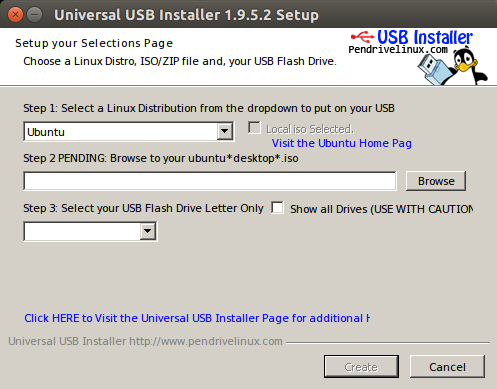
\includegraphics[width=\linewidth]{images/instalacja_nagrywanie_obrazu.png}
\end{wrapfigure}
\noindent Jeżeli chcesz użyć pendriva jako nośnika instalacyjnego to upewnij się iż ma on przynajmniej 1 gigabajt pojemności. W przeciwnym wypadku instalator nie zmiejści na nim. Jeżeli masz już przygotowany pendrive, wykonaj co następuje:
\begin{enumerate}
%TODO dla tej listy użyć włąsnych znaczników (label) przypominających te użyte na obrazkach.
\item Pobierz program \href{http://www.pendrivelinux.com/downloads/Universal-USB-Installer/Universal-USB-Installer-1.9.5.2.exe}{Universal USB Installer}.
\item Uruchom pobrany plik.
\item Zaakecptuj umowę licencyjną.
\item Podłącz do komputera pendrive, który ma użyty jako nośnik.
\item Z tej listy wybierz Ubuntu.
\item Kliknij na przycisk Browse i wskaż pobrany wcześniej obraz instalatora Ubuntu.
\item Z tej listy wybierz wczesniej podłączony pendrive.\\
\textbf{UWAGA: Wszystkie dane na nim zostaną skasowane!}
\item Kliknij przycisk CREATE.
\item Poczekaj na zakończenie operacji.
\end{enumerate}
\clearpage
\subsubsection{System Windows 7 / 8, nagrywanie na płytę DVD}
%TODO zweryfikować, czy windows 8 też to ma
\begin{wrapfigure}{r}{0.5\textwidth}
		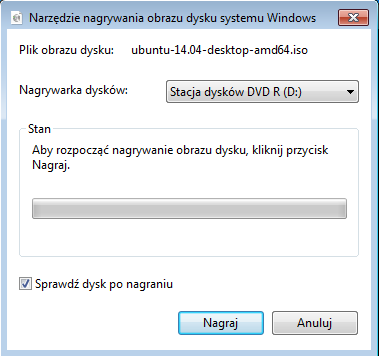
\includegraphics[width=\linewidth]{images/instalacja_nagrywanie_obrazu_DVD.png}
\end{wrapfigure}
Systemy operacyjne Windows 7 i 8 mają wbudowane narzędzie do wypalania plików .iso na płytach. Kliknij prawym przyciskiem myszy na pobrany obraz instalatora Ubuntu, wybierz opcję "Otwórz w" a następnie "Windows Disc Image Burner".
\begin{enumerate}
%TODO dla tej listy użyć włąsnych znaczników (label) przypominających te użyte na obrazkach.
%TODO jak to się po polsku nazywa?
\item Z tej listy wybierz swoją nagrywarkę.
\item Włóż czystą płytę DVD na wybranego napędu.
\item Upewnij się, że zaznaczone jest pole "Zweryfikuj dysk po nagraniu"
\item Kliknij na przycisk \textbf{Nagraj}
\end{enumerate}
\clearpage
\subsubsection{System Windows XP i inne starsze wersje, nagrywanie na płytę DVD}
\begin{wrapfigure}{R}{0.5\linewidth}
		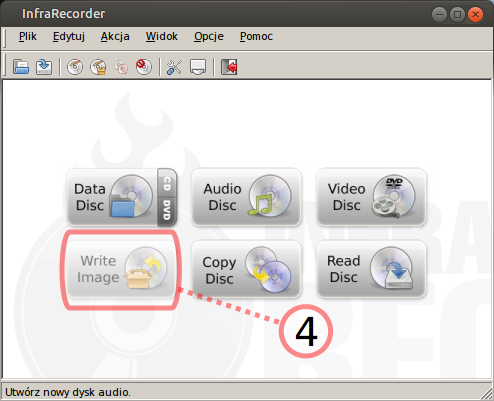
\includegraphics[width=\linewidth]{images/instalacja_nagrywanie_obrazu_DVD_winXP.png}
\end{wrapfigure}
Starsze wersje systemu Windows nie mają wbudowanej możliwości nagrywania płyt DVD. Potrzebne będzie do tego osobne narzędzie, program służący do wypalania płyt. Obsługa tych programów jest bardzo podobna: należy wybrać opcję \emph{Nagrywanie obrazu na płytę}. Koniecznie nagrywaj z wykorzystaniem tej opcji, gdyż inne (np.\emph{Nagrywanie płyty z danymi} lub \emph{Tworzenie kopi zapasowej}) utworzy dysk, którego twój komputer nie będzie potem wstanie uruchomić. Dla przykładu posłużymy się programem Infra Recorder.

\begin{enumerate}
\item Pobierz i zainstaluj program \href{http://infrarecorder.org/?page_id=5}{Infra Recorder}.
\item Uruchom nowozainstalowany program.
\item Włóż czystą płytę DVD do nagrywarki.
\item W programie Infra Recorder wybierz opcję \textbf{Write Image}.
\item Wybierz pobrany wcześniej obraz instalatora Ubuntu.
\item Kliknij na przycisk \textbf{OK}.
\end{enumerate}
\clearpage











		\subsubsection{System Linux, nagrywanie na pendriva}
\begin{wrapfigure}[6]{r}{0.5\textwidth}
                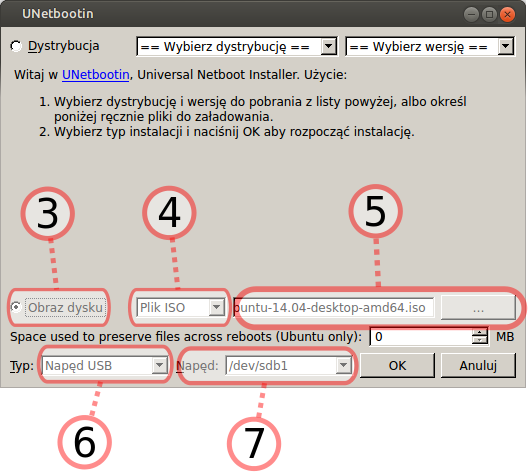
\includegraphics[width=\linewidth]{images/instalacja_nagrywanie_obrazu_linux.png}
\end{wrapfigure}

W systemach operacyjnych Linux do nagrywania obrazu na pendrive'a najlepiej posłużyć się programem \textcolor{ubuntu_orange}{UNetbootin}, dostępnym w każdej dystrybucji. Podłącz do komputera klucz USB, z którego chcesz potem instalować Ubuntu.
\begin{enumerate}[label=\protect\circled{\arabic*}]
\item Zainstaluj UNetBootIn korzystając ze swojego menadżera pakietów.
\item Uruchom zainstalowany przed momentem program.
\item Zaznacz pole Obraz dysku
\item Z menu wybierz Plik ISO
\item W tym polu podaj ścieżkę do pobranego wcześniej obrazu instalatora Ubuntu. Wciśnij przycisk oznaczony trzema kropkami (“\ldots”) i wskaż plik.
\item W tym menu wybierz Napęd USB
\item Z tego menu wybierz podłączonego wcześniej pendriva.\\
\textbf{UWAGA: Wszystkie dane znajdujące się na tym nośniku zostaną skasowane!}
\item Kliknij przycisk OK aby rozpocząć nagrywanie
\end{enumerate}
\subsubsection{System Linux, nagrywanie na DVD}
%TODO potrzebny obrazek z włożoną płytą DVD i wybranym obrazem ubuntu 14.04
\begin{wrapfigure}{l}{0.5\textwidth}
                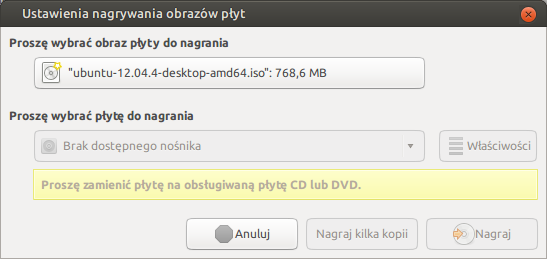
\includegraphics[width=\linewidth]{images/instalacja_nagrywanie_obrazu_linux_DVD.png}
\end{wrapfigure}

Aby nagrać obraz na płytę DVD potrzebujesz odpowiedniego programu. W tym przykładzie posłużymy się dostępną w większości dystrybucji nagrywarką Brasero. Kliknij prawym przyciskiem myszy na pobrany wcześniej obraz instalatora Ubuntu, wybierz \textcolor{ubuntu_orange}{Otwórz w\ldots}, a następnie wybierz \textcolor{ubuntu_orange}{Brasero}. W otwartym oknie zostaniesz poproszony o włożenie czystej płyty DVD. Zrób to, a następnie kliknij na przycisk \textcolor{ubuntu_orange}{Nagraj}.
\clearpage

	\subsection{Przygotowanie do instalacji}
		\subsubsection{Przygotowanie do instalacji - Windows - wskazówki ogólne}
\label{sec:przygotowanie_windows}
Instalując inny system operacyjny na dysku twardym swojego komputera zawsze istnieje ryzyko utraty danych. Wiele rzeczy może się zdażyć. Utrata zasilania w czasie partycjonowania dysku twardego najczęściej prowadzi do utraty jesgo zawartości. Przez zwykłą nieuwagę można nadpisać jede system drugim i w ten sposób utracić dane. Dlatego nim przystąpisz do instalacji systemu ubuntu upewnij się iż wszystkie wazne dane zostały zabezpieczone na zewnętrznych nośnikach danych. Innymi słowy: zrób kopię zapasową.

Warto też wyeksportować dane z programów takich jak przeglądarka internetowa(zakładki), klient pocztowy(konta, kalendarze i kontakty) i komunikator internetowy(konta, historia rozmów, znajomi). Nie zapomniej zrobić kopi zapasowej dokumentów czy swojej kolekcji muzyki. Jeżeli zainstalujesz Ubuntu obok Windowsa, to będziesz mieć dostęp do swoich plików. Niestety, w drugą stronę to nie działa i na systemach Windows nie ma możliwości podglądu plików na partycjach systemów Linuksowych\footnote{To jest możliwe, ale dosyć skomplikowane i wykracza poza zakres tego przewodnika}.

Ważnym krokiem jest ustalenie czy twoja płyta główna obsługiwana jest przez UEFI i jeżeli tak to jakie opcje są włączone. W konsoli systemu Windows (Start $\rightarrow$ Uruchom $\rightarrow$ cmd) wpisz \textit{Confirm-SecureBootUEFI}. System może zwrócić jedną z trzech informacji:
\begin{itemize}
\item \textit{Cmdlet not supported on this platform} lub \textit{Polecenia nie znaleziono} - Ten komputer nie korzysta z SecureBoot. Nie potrzebujesz nic więcej robić, wystarczy włożyć przygotowany nośnik instalacyjny i zainstalowac Ubuntu.
\item \textit{False} - Ten komputer na UEFI, ale nie korzysta z SecureBoot. Przejdź do sekcji porad dla Windows 8
\item \textit{True} - Ten komputer na UEFI, ale korzysta z SecureBoot. Przejdź do sekcji porad dla Windows 8
\end{itemize}
\subsubsection{Przygotowanie do instalacji - Windows 8}
\label{sec:przygotowanie_windows8}
Windows 8 wymusił na producentach sprzetu stosowanie technologi UEFI (zamiast BIOSu) oraz SecureBoot(Zabezpieczenie komputera przed zmianami systemu operacyjnego), co znacznie utrudniło instalację innych systemów operacyjnych. Ubuntu jest przygotowane do współpracy z Windowsem 8, ale Windows nie jest przygotowany do współdzielenia komputera z innymi systemami operacyjnymi. Pamiętaj, że jeżeli posiadasz UEFI (a używanie Windows 8 na to wskazuje) to potrzebujesz Ubuntu w wersji 64 bitowej. Systemy 32 bitowe nie są obsługiwane przez technologię UEFI\footnote{A przynajmniej nie bez dużej ilości kombinowania}.

W tym momencie warto przygotować wolną przestrzeń na dysku pod instalację Ubuntu. Ten punkt można wykonać zarówno teraz jak i podczas instalacji Ubuntu, jednak jeżeli używasz Windows 8 lepiej zrobić to teraz. Wciśnij kombinację klawiszy super + r i uruchom program compmgmt.msc. W uruchomionym programie utwórz partycję dla Ubuntu. Absolutne minimum dla tej partycji to 8 gigabajtów. Ubuntu potrzebuje około 4 gigabajtów na podstawową instalację, pozostałe miejsce będzie można przeznaczyć na instalację oprogramowania oraz pliki uzytkownika. Zalecamy jednak stworzneie przynajmniej 20 gigabajtowej partycji.

Windows 8 korzysta z opcji Szybkiego Uruchamiania (Fast Boot), która to uniemożliwia dostęp do plików Windowsa przez system Ubuntu. Jedynym sposobem na obejście tego jest wyłączenie opcji Szybkiego uruchamiania. Wejdź w Panel Sterowania, następnie Opcje Zasilania a potem Wybierz co ma robić przycisk zasilania. Odhacz opcję "Włącz Szybkie uruchamiania (zalecane)".

\subsubsection{Przygotowanie do instalacji - Linux}
\label{sec:przygotowanie_linux}
Instalacja jednego systemu Linux obok drugiego nie powoduje zadnych problemów, jednak powinieneś wiedzieć o paru sprawa. W Linuksach pliki użytkownika są przechowywane w katalogu /home. Dobrą praktyką jest wydzielenie osobnej partycji dla tego katalogu, aby przy reinstalacji systemu nie tracić swoich ustawień. Jeżeli instalujesz jednego Linuksa obok drugiego to kuszącym może być wykorzystanie jednej partycji domowej dla obu systemów. 
To jest możliwe, ale weź pod uwagę iż różne systemy mogą korzystać z różnych plików - nie wszystkie ustawienia będą widoczne na obu systemach (szczególnie jeżeli korzystasz z różnych środowisk graficznych). Przy takiej konfiguracji ważne jest też aby nazwa użytkownika oraz jego grupy były taka sama na obu systemach.
Jeżeli systemy, które instalujesz obok siebie bardzo się różnią, to lepiej nie korzystać ze wspólnego katalogu domowego, a ze wspólnych dokumentów, filmów czy muzyki korzystać za pomocą wspólnego katalogu.

Potrzebujesz tylko jednej partycji wymiany (swap) niezależnie od tego ile systemów instalujesz.
	\subsection{Uruchomienie instalatora}
		\subsubsection{Ponowne uruchomienie komputera}
Jeżeli dysponujesz już  nośnikiem instalacyjnym, nie pozostaje nic innego, jak uruchomić instalator i zainstalować system na dysku twardym komputera. Jeśli korzystasz z tego przewodnika w trybie online, dobrym pomysłem będzie wydrukowanie kilku kolejnych stron. Może się zdarzyć, że w czasie instalacji stracisz dostęp do internetu i zostaniesz tym samym odcięty od zawartych tutaj informacji.

Przed przystąpieniem do instalacji koniecznie zapoznaj się także z następującymi sekcjami:
\begin{itemize}
\item \ref{sec:przygotowanie_windows} \textit{Przygotowanie do instalacji - Windows - wskazówki ogólne}: ta sekcja zawiera przydatne informacje dla osób migrujących z systemów Windows.
\item \ref{sec:przygotowanie_windows8} \textit{Przygotowanie do instalacji - Windows 8}: pecyficzne porady dla systemu Windows 8. Koniecznie ten fragment przewodnika, jeżeli instalujesz Ubuntu obok Windows 8 lub próbujesz zainstalować Ubuntu zamiast Windows 8.
\item \ref{sec:przygotowanie_linux} \textit{Przygotowanie do instalacji - Linux}: ogólne wskazówki dla osób instalujących Ubuntu obok innych dystrybucji Linuksa.
\end{itemize}
Zrestartuj swój komputer i uruchom go z przygotowanego nośnika instalacyjnego. W większości przypadków wiąże się to z ręcznym wskazaniem odpowiedniego napędu podczas uruchamiania komputera. Jeśli twój komputer wyposażony jest w system UEFI, cała ta procedura będzie znacznie bardziej skomplikowana.

\subsubsection{Zmiana kolejności bootowania}
Kiedy rozpocznie się rozruch komputera, jeszcze przed załadowaniem się systemu operacyjnego musisz poinformować maszynę, że tym razem  zamiast systemu zainstalowanego na twardym dysku ma ona wykorzystać przygotowany przez nas instalator. Każdy producent płyt głównych podchodzi do tej kwestii w nieco odmienny sposób, jednak najczęściej procedura będzie się pokrywać z jednym z opisanych poniżej scenariuszy:
\begin{itemize}
\item Niektóre komputery podczas rozruchu pokazują napis Press F12 to select boot device. Kluczowymi słowami są tutaj ”Boot Device”, ”Boot order” lub podobne . Wciśnij wskazany klawisz (w tym konkretnym przypadku F12, ale nie jest to reguła) i z wyświetlonego menu wybierz nośnik instalacyjny. Niektóre komputery wykrywają pendrive'y jako dyski twarde i musisz wskazać właśnie taki dysk twardy a nie port USB. Jeżeli na liście nie ma naszego instalatora, zresetuj komputer i spróbuj ponowanie.
\item Jeżeli zobaczysz napis \textbf{Press ESC to enter setup} lub coś podobnego, twoim słowem kluczowym będzie ”setup”. Wciśnięcie odpowiedniego klawisza (ESC, delete lub któryś z klawiszy funkcyjnych) spowoduje uruchomienie programu konfiguracyjnego płyty głównej. W tym programie przejdź do sekcji ”Advanced BIOS Features” a następnie ”First Boot Device”. Wskaż napęd CD-ROM lub napęd USB (względnie drugi dysk twardy, jeżeli pendrive jest rozpoznawany jako dysk twardy). Wróć do menu głównego (klawisz ESC cofa o jedno menu) i zapisz zmainy (najczęściej F10, czasem ESC i potwierdzenie przy pomocy klawisza Y). W tym momencie komputer samoczynnie się zrestartuje.
\end{itemize}
\subsubsection{Uruchomienie instalatora UEFI}
Po wybraniu urządzenia z nośnikiem instalacyjnym komputer rozpocznie proces jego uruchamiania. Może to potrwać od kilku do kilkunastu sekund. W tym czasie ekran komputera będzie czarny bądź będą się przez niego przewijały napisy.\\
Jeżeli twoja maszyna pracuje pod kontrolą UEFI, to pierwszy ekran instalatora będzie wyglądał jak na poniższym rysunku:
\begin{center}
	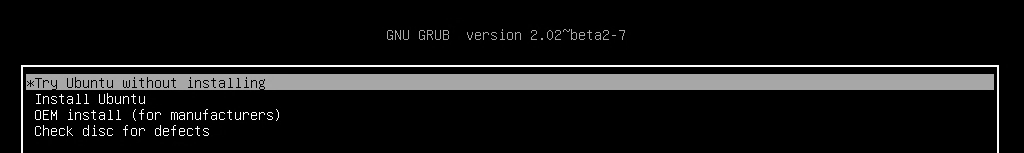
\includegraphics[width=\linewidth]{images/instalacja_UEFI_boot.png}
\end{center}
Do wyboru masz następujące opcje:
\begin{description}
\item[Try Ubuntu without installing](Wypróbuj Ubuntu bez instalowania) - Uruchomi system Ubuntu bez instalacji go na dysku twardym. W ten sposób możesz przetestować Ubuntu i zobaczyć jak działa w praktyce. Wszystkie zmiany jakie wprowadzisz w systemie zostaną odrzucone po wyłączeniu komputera. Należy pamiętać, że w tym trybie Ubuntu działa bardzo wolno, gdyż musi korzystać z powolnego nośnika (płyta DVD lub pendriva). Po normalniej instalacji ubuntu będzie działać z pełną wydajnością. Skrót do instalatora systemu znajduje się na Pulpicie.
\item[Install Ubuntu](Zainstaluj Ubuntu) - Ta opcja bezpośrednio uruchomi instalator Ubuntu bez wczytywania całego systemu.
\item[OEM Install](Instalacja dla producentów sprzętu) - Ta opcja pozwala zainstalować podstawowy system bez tworzenia użytkownika. Przy pierwszym uruchomieniu zostaniesz poproszony o stworzenie nowego użytkownika.
\item[Check disk for defects](Sprawdź płytę pod kontem błędów odczytu) - Ta opcja sprawdzi czy używany nośnik został prawidłowo utworzony.\\
Przed przystąpieniem do instalacji systemu warto wykonać sprawdzenie nośnika instalacyjnego. Potrwa to góra kilka minut a pozwoli zaoszczędzić czas w przyszłości. Podczas przeprowadzania testów komputer może wyświetlać tylko czarny ekran. Jeżeli nie znajdzie żadnych błędów, otrzymasz komunikat "Check Finished: No errors found. Press any key to reboot your system" (Zakończono sprawdzanie: Nie znaleziono błędów.Wciśnij dowolny klawisz aby zresetować komputer). Po ponownym uruchomieniu komputera możesz przystąpić do instalacji. Jeżeli znaleziono jakiekolwiek błędy to należy ponownie przygotować nośnik instalacyjny. Uzycie wadliwego instalatora doprowadzi do uszkodzenia systemu. 
\end{description}

\subsubsection{Uruchomienie instalatora BIOS}
\begin{wrapfigure}{L}{0.4\textwidth}
		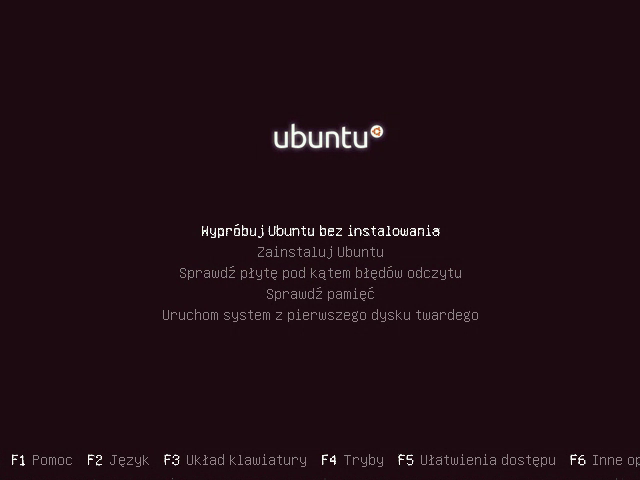
\includegraphics[scale=0.5]{images/instalacja_BIOS_boot.png}
\end{wrapfigure}
Po wybraniu urządzenia z nośnikiem instalacyjnym komputer rozpocznie proces jego uruchamiania. Może to potrwać od kilku do kilkunastu sekund. W tym czasie ekran komputera będzie czarny bądź będą się przez niego przewijały napisy. Kiedy ekran komputera zmieni kolor z czarnego na fioletowy wciśnij dowolny klawisz aby wejść do ustawień instalatora. Jeżeli tego nie zrobisz, komputer uruchomi instalator z domyślnymi opcjami.Na początek wybierz język w jakim system bedzie się z toba komunikował. Przy pomocy klawiszy kursora przejdź do trzeciej kolumny. Język Polski  znajduje się mniej więcej w połowie tej kolumny. Wciśnij enter aby zatwierdzić.
\clearpage
\begin{description}
\item[Wypróbuj Ubuntu bez instalowania] - Uruchomi system Ubuntu bez instalacji go na dysku twardym. W ten sposób możesz przetestować Ubuntu i zobaczyć jak działa w praktyce. Wszystkie zmiany jakie wprowadzisz w systemie zostaną odrzucone po wyłączeniu komputera. Należy pamiętać, że w tym trybie Ubuntu działa bardzo wolno, gdyż musi korzystać z powolnego nośnika (płyta DVD lub pendriva). Po normalniej instalacji ubuntu będzie działać z pełną wydajnością. Skrót do instalatora systemu znajduje się na Pulpicie.
\item[Zainstaluj Ubuntu] - Ta opcja bezpośrednio uruchomi instalator Ubuntu bez wczytywania całego systemu.
\item[Sprawdź płytę pod kontem błędów odczytu] - Ta opcja sprawdzi czy używany nośnik został prawidłowo utworzony.\\
Przed przystąpieniem do instalacji systemu warto wykonać sprawdzenie nośnika instalacyjnego. Potrwa to góra kilka minut a pozwoli zaoszczędzić czas w przyszłości. Podczas przeprowadzania testów komputer może wyświetlać tylko czarny ekran. Jeżeli nie znajdzie żadnych błędów, otrzymasz komunikat "Check Finished: No errors found. Press any key to reboot your system" (Zakończono sprawdzanie: Nie znaleziono błędów.Wciśnij dowolny klawisz aby zresetować komputer). Po ponownym uruchomieniu komputera możesz przystąpić do instalacji. Jeżeli znaleziono jakiekolwiek błędy to należy ponownie przygotować nośnik instalacyjny. Uzycie wadliwego instalatora doprowadzi do uszkodzenia systemu. 
\item[Sprawdź pamięć] - Ta opcja uruchomi program memtest, który wykona test pamięci operacyjnej komputera (RAM). Uszkodzona pamięć jest jedną z częstrzych przyczyn błędów instalatora jak i wpływa negatywnie na pracę zainstalowanego systemu.
\item[Uruchom system z pierwszego dysku twardego] - Ta opcja kończy pracę instalatora i uruchamia podstawowy system operacyjny komputera.
\end{description}
Dodatkowe opcje widoczne na dolnym pasku uruchamia się wciskając odpowiedni klawisz funkcyjny:
\begin{description}
\item[F1] - Wyświetla pomoc, wraz z szczegółowym opisem poszczególnych opcji konfiguracyjnych.
\item[F2] - Zmiana języka instalatora.
\item[F3] - Zmiana układu klawiatury.
\item[F4] - Zmiana trybu pracy instalatora.
	\begin{description}
	\item[Zwykły] - Tryb podstawowy, teraz się w nim znajdujesz
	\item[Użycie nośnika aktualizującego sterowniki] - ??
	\item[Instalacja OEM(dla producentów sprzętu)] - Ta opcja pozwala zainstalować podstawowy system bez tworzenia użytkownika. Przy pierwszym uruchomieniu zostaniesz poproszony o stworzenie nowego użytkownika.
	\end{description}
\item[F5] - Pozwala włączyć/wyłączyć dodatkowe opcje ułatwiające instalacje osobom niepełnosprawny (Klawiatura ekranowa, lupa, wyski kontrast, czytnik ekranu, klawiatura Braille'a)
\item[F6] - Dodatkowe parametry rozruchu, pomocne w przypadku napotkania problemów ze sprzetem.
\end{description}
\clearpage


	\subsection{Graficzny instalator Ubuntu}
		Niezależnie od tego, czy posiadasz płytę główną z BIOS-em, czy z UEFI, w poprzednim punkcie powinieneś wybrać \textcolor{ubuntu_orange}{Zainstaluj Ubuntu}. Ta metoda jest szybsza od \textcolor{ubuntu_orange}{Wypróbuj Ubuntu bez instalowania}, gdyż nie wymaga załadowania całego systemu. Jeżeli mimo wszystko uruchomiłeś cały system w trybie Live, to na pulpicie znajdziesz ikonę \textcolor{ubuntu_orange}{Zainstaluj Ubuntu} (lub ,,Install Ubuntu'', jeżeli nie zmieniałeś języka). Od tego momentu instalacja przebiega w identyczny sposób dla każdego wybranego sposobu instalacji.

W czasie instalacji w prawej części paska u góry ekranu znajduje się szerego ikon:
\begin{description}
\item[
\includegraphics{images/ikony_dostempnosc.png}]\textcolor{ubuntu_orange}{Dostępność} --- uruchomienie lupy, czytnika ekranowego lub klawiatury ekranowej.
\item[
\includegraphics{images/ikony_internet.png}]\textcolor{ubuntu_orange}{Łączność} --- konfiguracja połączenia z internetem na czas instalacji systemu.
\item[
\includegraphics{images/ikony_jezyk.png}]\textcolor{ubuntu_orange}{Język} --- zmiana języka oraz układu klawiatury na czas instalacji systemu.
\item[
\includegraphics{images/ikony_dzwiek.png}]\textcolor{ubuntu_orange}{Ustawienia głośności i dźwięku}
\item[
\includegraphics{images/ikony_zasilanie.png}]\textcolor{ubuntu_orange}{Zasilanie} --- wyłączenie lub ponowne uruchomienie komputera.
\end{description}
\clearpage
\subsubsection{Wybór języka}
\begin{center}
        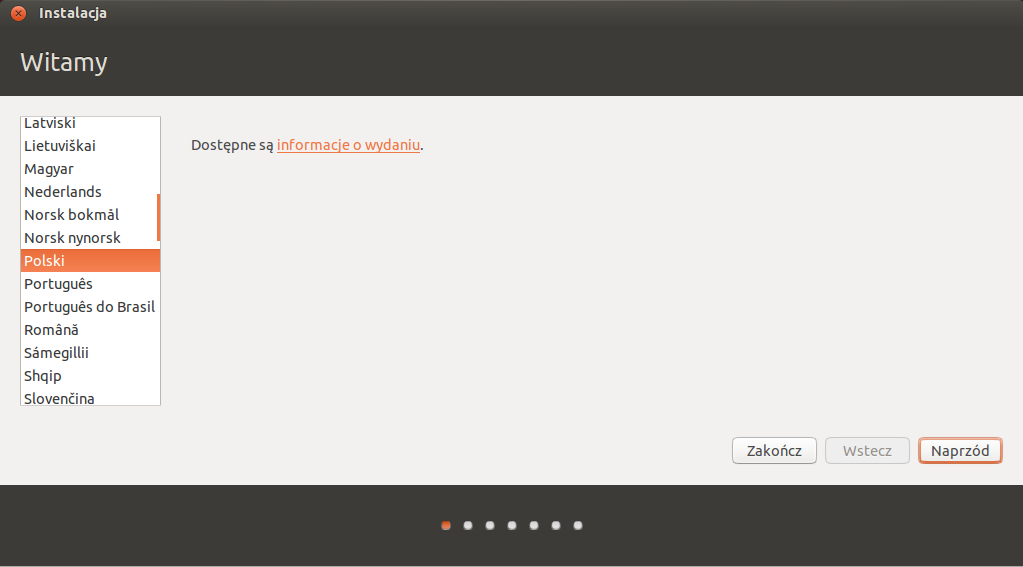
\includegraphics[width=\linewidth]{images/instalator_jezyk.png}
\end{center}

Pierwszy ekran instalatora pozwala wybrać język. Jeżeli wcześniej nie zmieniłeś języka na polski, to teraz masz ku temu okazję. Język wybrany podczas instalacji będzie także domyślnym językiem zainstalowanym w systemie.
\begin{flushright}
Kliknij przycisk \textcolor{ubuntu_orange}{Naprzód}, aby przejść dalej.
\end{flushright}
\clearpage
\subsubsection{Konfiguracja Wi-Fi}
\begin{center}
        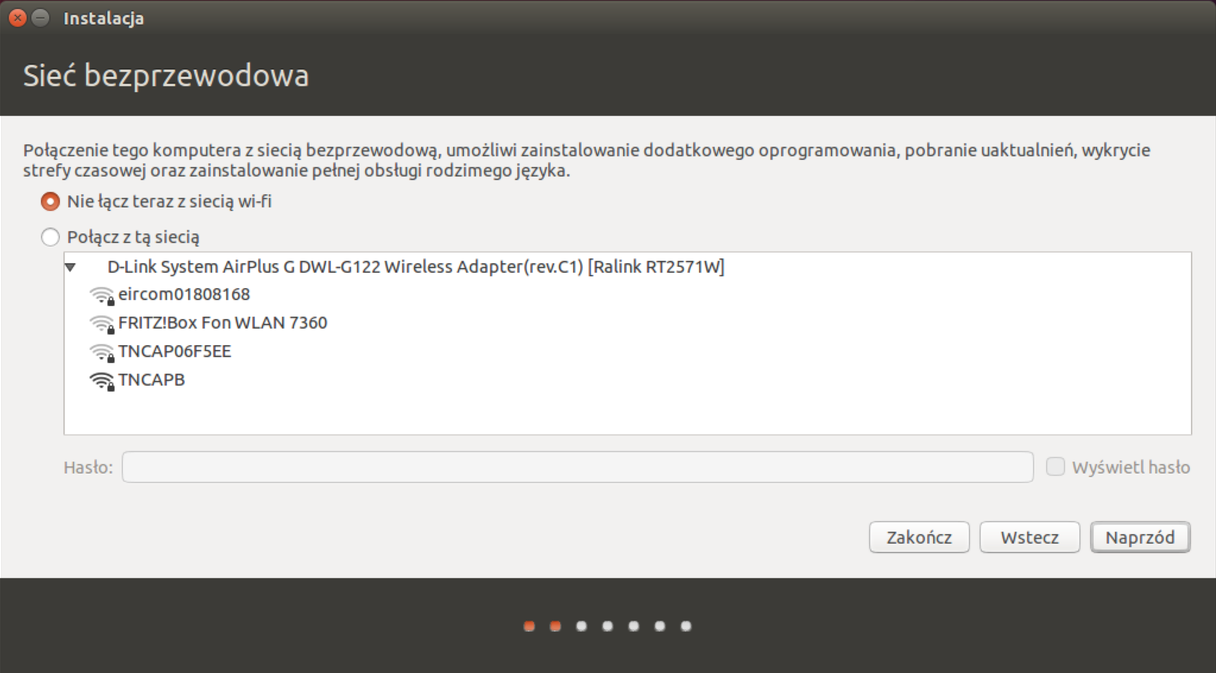
\includegraphics[width=\linewidth]{images/instalator_wifi.png}
\end{center}

Drugi ekran instalatora pozwala skonfigurować połączenie bezprzewodowe Wi-Fi. Jeżeli instalator nie wykryje żadnej karty Wi-Fi, to nie pokaże tego ekranu. Ten etap instalacji zostanie pominięty również wtedy, gdy uda się nawiązać połączenie przewodowe.

Z listy na ekranie wybierz sieć bezprzewodową, z którą chcesz się połączyć. Wpisz hasło do sieci bezprzewodowej w pole \textcolor{ubuntu_orange}{Hasło}.
\begin{flushright}
Kliknij przycisk \textcolor{ubuntu_orange}{Naprzód}, aby przejść dalej.
\end{flushright}
\clearpage
\subsubsection{Sprawdzenie kompatybilności sprzętu, wybór dodatkowych komponentów}
\begin{center}
        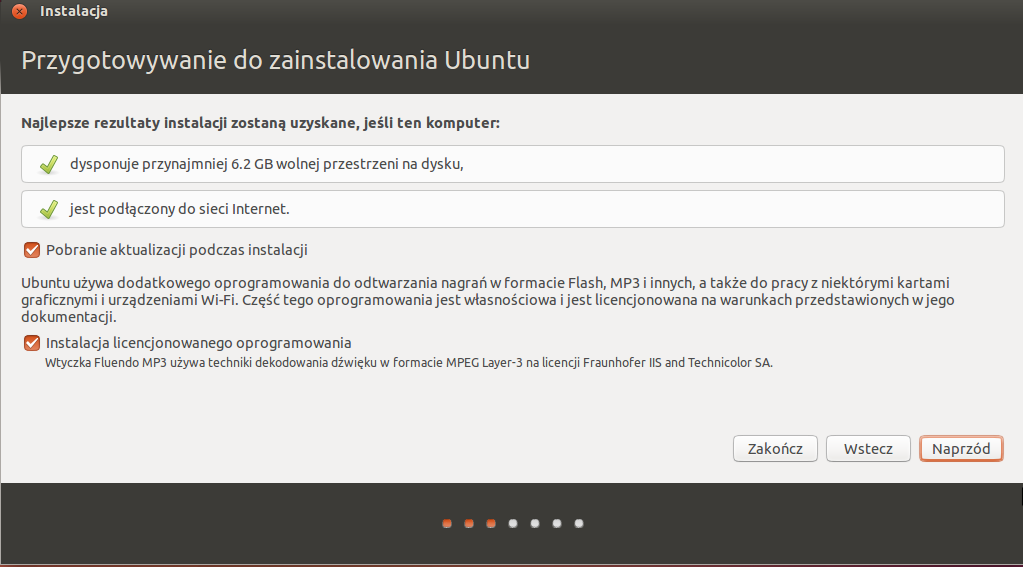
\includegraphics[width=\linewidth]{images/instalator_wymagania.png}
\end{center}

Na tym etapie instalator sprawdzi, czy na dysku twardym jest wystarczająco dużo miejsca, aby zainstalować Ubuntu. Połączenie z internetem nie jest wymagane do zainstalowania systemu, jest jednak niezbędne, by zainstalować spolszczenie, aktualizacje oraz dodatkowe wtyczki. Jeżeli w tym momencie nie masz połączenia z internetem, to pobranie paczek lokalizacyjnych będzie możliwe później. Zostało to opisane w rozdziale \ref{rzeczy_do_zrobienia_po_instalacji} ,,Rzeczy do zrobienia po instalacji Ubuntu''.
\begin{itemize}
\item \textcolor{ubuntu_orange}{Pobieranie aktualizacji podczas instalacji} --- Instalator pobierze i zainstaluje wszystkie aktualizacje, które zostały wydane od dnia premiery systemu.
\item \textcolor{ubuntu_orange}{Instalacja licencjonowanego oprogramowania} --- W skład pakietu wchodzą własnościowe sterowniki do kart graficznych AMD lub Nvidii, sterowniki do kart Wi-Fi, kodeki audio-wideo (po instalacji Ubuntu będzie w stanie odtworzyć prawie każdy rodzaj plików muzycznych i filmowych) oraz wtyczka Flash do przeglądarki internetowej.
\end{itemize}
\begin{flushright}
Kliknij przycisk \textcolor{ubuntu_orange}{Naprzód}, aby przejść dalej.
\end{flushright}
\clearpage
\subsubsection{Partycjonowanie dysku twardego}
\begin{center}
        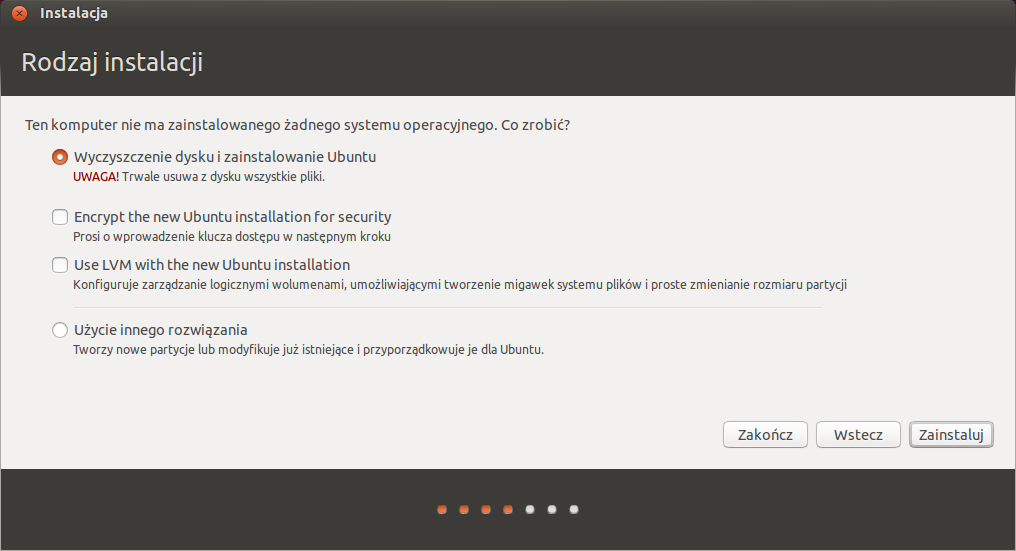
\includegraphics[width=\linewidth]{images/instalator_partycjonowanie_proste.png}
\end{center}

Jest to najważniejszy etap instalacji. W tym miejscu można dokonać cudów, jak i zniszczyć cały dysk twardy. Jako że prawidłowe partycjonowanie dysku twardego to bardzo szeroki temat, to poświęciliśmy mu cały osobny rozdział. Na powyższym obrazie widać najprostszą wersję tego etapu instalacji. Na dysku twardym nie ma zainstalowanego żadnego systemu operacyjnego i instalator proponuje wykorzystanie całej przestrzeni dla Ubuntu. Jeżeli masz inne systemy operacyjne, to instalator zaproponuje wydzielenie miejsca i instalację Ubuntu obok danego systemu operacyjnego. Jeżeli miałeś wcześniej zainstalowane Ubuntu, instalator zaproponuje aktualizację do najnowszego wydania lub usunięcie i zainstalowanie Ubuntu ponownie.
Partycjonowanie zostało szeroko opisane w rozdziale \ref{subsec:partycjonowanie} ,,Zaawansowane partycjonowanie''. Wróć tutaj, gdy go przeczytasz.
\begin{flushright}
Kliknij przycisk \textcolor{ubuntu_orange}{Naprzód}, aby przejść dalej.
\end{flushright}
\clearpage
\subsubsection{Wybór strefy czasowej}
\label{instalator_strefa_czasowa}
\begin{center}
        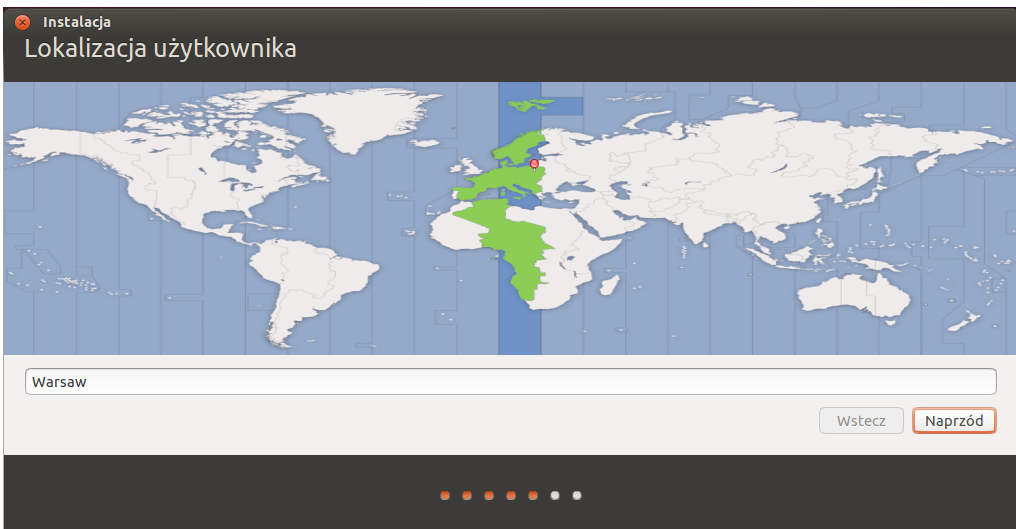
\includegraphics[width=\linewidth]{images/instalator_czas.png}
\end{center}

Na tym etapie należy wybrać lokalizację tego komputera, aby system mógł wyświetlać prawidłowy czas i automatycznie dostosowywać się do zmian pomiędzy czasem letnim i zimowym. Jeżeli w trakcie instalacji masz połączenie z internetem, to odpowiednia lokalizacja zostanie wybrana automatycznie. Jeżeli nie masz dostępu do internetu, w pole wpisz \textcolor{ubuntu_orange}{Warsaw}. Stolica naszego kraju określa też naszą strefę czasową.
\begin{flushright}
Kliknij przycisk \textcolor{ubuntu_orange}{Naprzód}, aby przejść dalej.
\end{flushright}
\clearpage
\subsubsection{Wybór układu klawiatury}
\begin{center}
        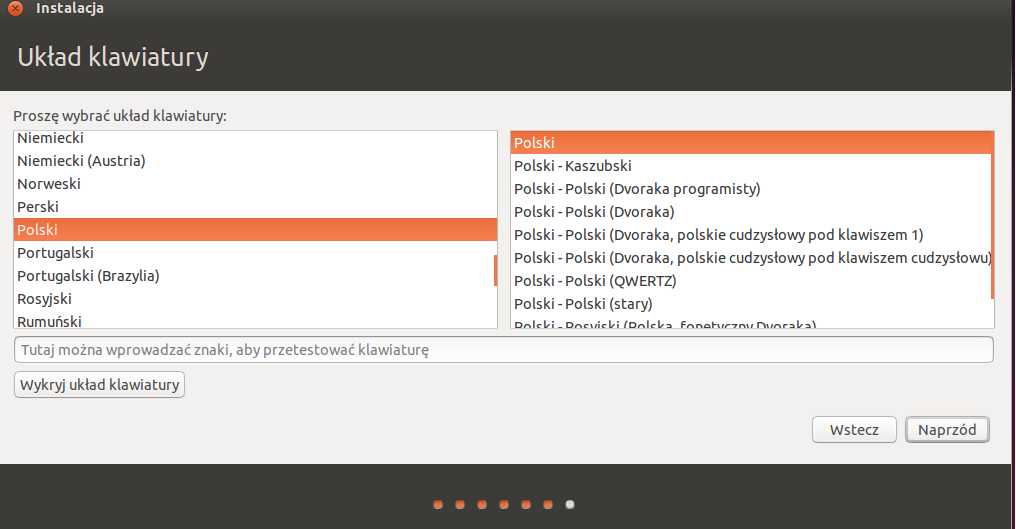
\includegraphics[width=\linewidth]{images/instalator_klawiatura.png}
\end{center}

Ten ekran pozwala wybrać układ klawiatury. Jeżeli wybrałeś wcześniej język polski, to standardowa polska klawiatura zostanie wybrana automatycznie. W polu możesz wpisać kilka znaków, aby sprawdzić, czy zaznaczony układ odpowiada rzeczywistości. Pierwsza opcja (\textcolor{ubuntu_orange}{Polski}) to standardowa klawiatura mieszcząca 101 klawiszy, zwana potocznie układem programisty.
Nie zalecamy korzystania z funkcji \textcolor{ubuntu_orange}{Wykryj układ klawiatury}. Korzystając ze wskazówek instalatora otrzymamy klawiaturę amerykańską, nieobsługującą polskich znaków diakrytycznych.
\begin{flushright}
Kliknij przycisk \textcolor{ubuntu_orange}{Naprzód}, aby przejść dalej.
\end{flushright}
\clearpage
\subsubsection{Tożsamość użytkownika}
\begin{center}
        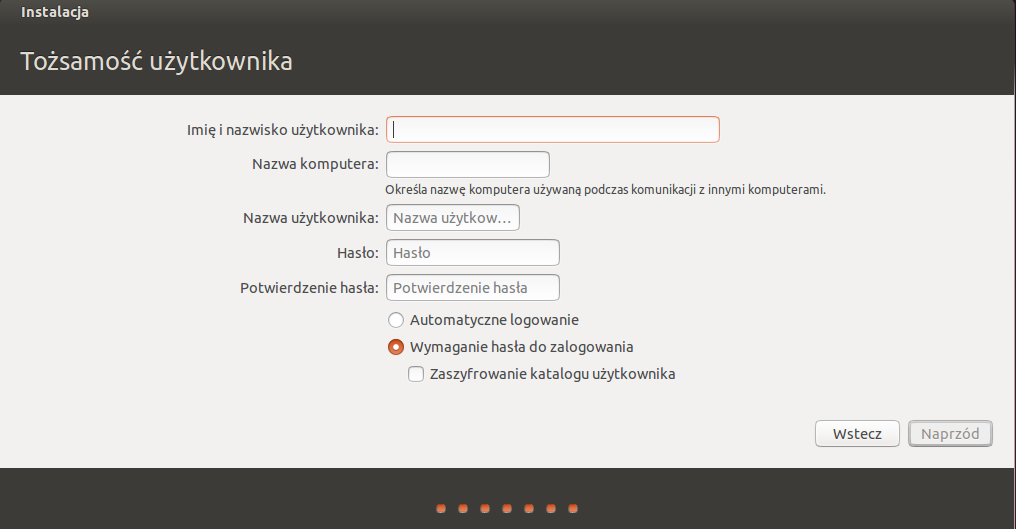
\includegraphics[width=\linewidth]{images/instalator_dane.png}
\end{center}

To już ostatni etap instalacji. Te pola należy uzupełnić, aby system mógł cię prawidłowo zidentyfikować.
\begin{itemize}
\item \textcolor{ubuntu_orange}{Imię i nazwisko użytkownika} --- Pole nieobowiązkowe, ale jeżeli uzupełnisz te dane, to system będzie się do ciebie zwracał imieniem i nazwiskiem, zamiast używać loginu (np. Jan Kowalski).
\item \textcolor{ubuntu_orange}{Nazwa komputera} --- Określa jak będzie się nazywał twój komputer (np. laptop).
\item \textcolor{ubuntu_orange}{Nazwa użytkownika} --- Twój login do systemu (np. jan\_kowalski albo twój pseudonim). Login nie może zawierać wielkich liter, spacji, ani znaków specjalnych.
\item \textcolor{ubuntu_orange}{Hasło} --- Hasło do komputera. Hasło zabezpiecza system przed nieuprawnionym dostępem.\\
Uwaga: Ustawienie hasła uniemożliwia innym zalogowanie się do twojego konta, jednak nie zabezpiecza twoich danych przed podejrzeniem przez inne osoby, o ile ich nie zaszyfrujesz. 
\item \textcolor{ubuntu_orange}{Potwierdzenie hasła} --- Wpisz ponownie to samo hasło, co w polu powyżej.
\item \textcolor{ubuntu_orange}{Automatyczne logowanie} --- Jeżeli zaznaczysz to pole, system automatycznie zaloguje tego użytkownika po uruchomieniu. Nie będzie potrzebne podawanie hasła, aby uzyskać dostęp do komputera.
\item \textcolor{ubuntu_orange}{Wymaganie hasła do zalogowania} --- Po uruchomieniu komputera będziesz musiał podać hasło, aby uzyskać dostęp do swojego konta.
\item \textcolor{ubuntu_orange}{Zaszyfrowanie katalogu użytkownika} --- Jeżeli zaznaczysz to pole, twoje prywatne dane zostaną zaszyfrowane. Nikt nieznający hasła nie będzie mógł uzyskać dostępu do twoich plików. Jeżeli zapomnisz hasło, to bezpowrotnie utracisz dostęp do swoich plików.
\end{itemize}
\begin{flushright}
Kliknij przycisk \textcolor{ubuntu_orange}{Naprzód}, aby przejść dalej.
\end{flushright}
\clearpage
\subsubsection{Instalacja}
\begin{center}
        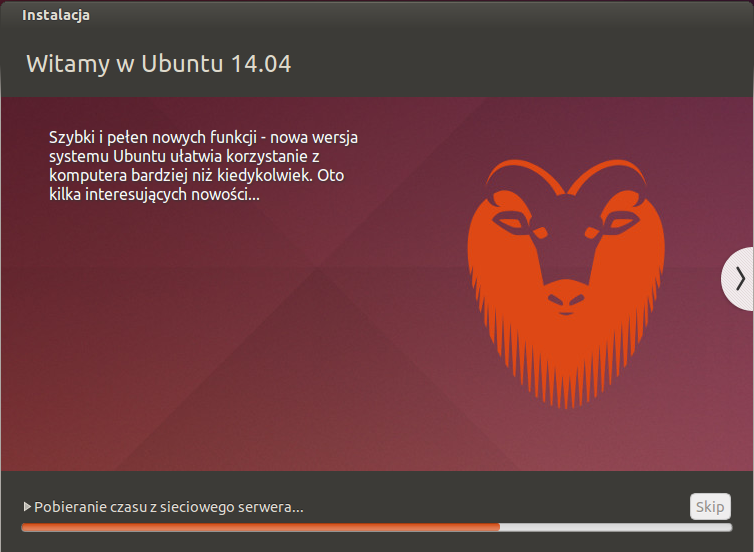
\includegraphics[width=\linewidth]{images/instalator_kopiowanie.png}
\end{center}

Teraz system dokona instalacji na dysku twardym oraz ewentualnie pobierze i zainstaluje paczki językowe, aktualizacje i dodatkowe oprogramowanie. Proces ten może potrwać od kilku, do kilkunastu minut w zależności od klasy komputera, ilości zadań do wykonania oraz szybkości łącza internetowego.
Po zakończeniu instalacji zostaniesz poproszony o usunięcie nośnika instalacyjnego i ponowne uruchomienie komputera. Jeżeli wszystko poszło pomyślnie, to za minutę zostaniesz przywitany pulpitem Ubuntu.
\begin{flushright}
\textcolor{ubuntu_orange}{Gratulacje!} Właśnie zainstalowałeś Ubuntu 14.04 LTS Trusty Tahr.\\
Komputer zostanie zresetowany.\\
Przejdź do sekcji \ref{pierwsze_uruchomienie}:,,Pierwsze Uruchomienie Ubuntu''.
\end{flushright}
\clearpage

	\subsection{Zaawansowane partycjonowanie}
		\label{subsec:partycjonowanie}
Patrycjonowanie to proces zmiany układu partycji na dysku twardym. Jest to najważniejszy etap instalacji systemu gdyż to od niego w dużej mierze zależy jak system będzie działał. Pamiętaj, że na tym etapie pracujesz na danych zapisanych na dysku twardym. Chwila nieuwagi może spowodować utratę jego zawartości.
\subsubsection{Ile miejsca przeznaczyć na Ubuntu}
\label{subsubsec:ile_miejsca}
Wirtualny dysk twardy użyty w tym przewodniku ma tylko 26.8 gigabajta pojemności. Twój dysk twardy będzie miał zapewne kilkaset gigabatów (jeżeli nie kilka terabajtów) pojemności. Dlatego też liczby jkimi się tu posługujemy będą miały niewielkie przełożenie na sytuację na twoim komputerze. W tym miejscu powinieneś się jednak zastanowić ile miejscach chcesz przeznaczyć na Ubuntu.

Ogólnie rzecz ujmując sprawa wygląda następująco
\begin{description}
\item[Partycja główna, root, /] - 6,2 Gigabajta to apsolutne minimum. 10 gigabajtów da pewną elastyczność i pozwoli zainstalować więcej programów. Nie ma potrzeby przesadzać w drugą stronę i tworzyć zbyt dużej partycji głównej, gdyż wolna przestrzeń będzie niewykorzystana. 15-20 gigabajtów w zupełności wystarczy.
\item[Partycja wymiany, swap] - na tej partycji zapisywane są dane, które nie mieszczą się w pamięci operacyjnej. Tutaj też przechowywany jest obraz RAMu kiedy poddajesz komputer hibernacji. Jeżeli korzystasz z hibernacji to wielkość partycji swap powinna być conajmniej taka jak ilość pamięci operacyjnej twojego komputera. Jeżeli nie planujesz korzystać z hibernacji to możesz nie tworzyć partycji wymiany. Jednak zaleca się jej stworzenie, jeżeli masz mniej niż 2 gigabajty RAMu. W takim wypadku nawet jeżeli nie korzystasz z hibernacji to dobrze jest stworzyć niewielką (300 - 400 megabajtów) partycję swap.
\item[Partycha domowa, /home] - W katalogu /home przechowywane są prywatne pliki użytkownika: zawartość pulpitu, dokumenty, filmy, muzyka i ustawienia programów. Katalog domowy może znajdować się na głównej partycji (/, root) lub można go wydzieć. Dobrą praktyką jest wydzielenie takiej partycji, gdyż w razie reinstalacji systemu nie trzeba będzie jej kasować. Nadpisana pozostanie tylko partycja główna, zaś wszystkie prywatne dane pozostaną niezmienione. Wielkość tej partycji zależy tylko i wyłącznie od tego jak wiele miejsca chcesz na nią przeznaczyć i jak wiele rzeczy zamierzasz na niej trzymać. 
\end{description}
\clearpage
\subsubsection{Czysty dysk - wykorzystanie całego dostępnego miejsca}
\begin{center}
	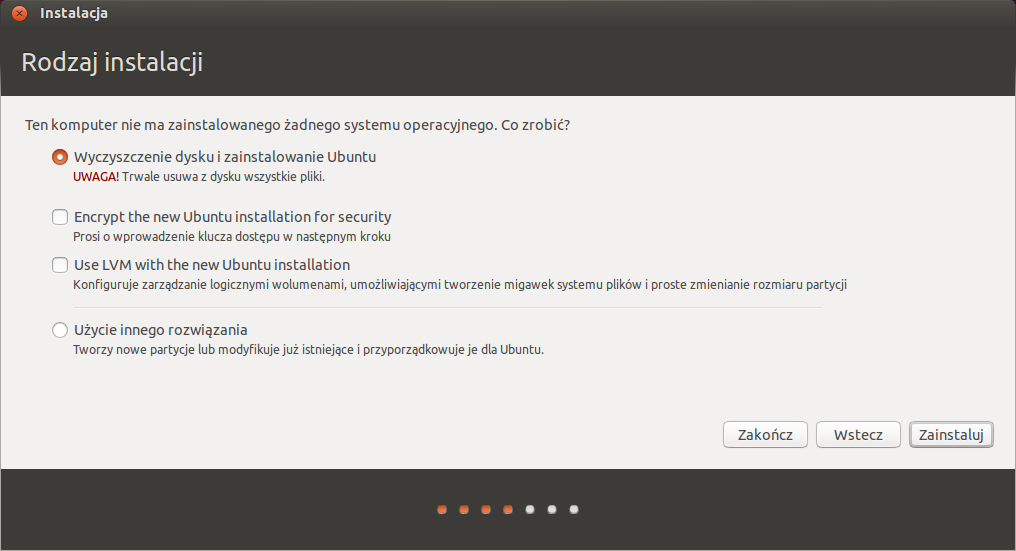
\includegraphics[scale=0.5]{images/instalator_partycjonowanie_proste.png}
\end{center}

Jeżeli na dysku twardym nie ma żadnego innego systemu operacyjnego, instalator ubuntu zaproponuje wykorzystanie całej dostępnej przestrzeni. Instalator sam dobierze odpowiedni rozmiar partycji systemowej, partycji wymiany oraz partycji użytkownika.
\begin{flushright}
Kliknij na przycisk \textbf{Zainstaluj} aby przejść dalej.\\
Zostaniesz poproszony o potwierdzenie. Upewnij się, że wszystko jest w pożądku i kliknij \textbf{Naprzód}.\\
W tym momencie wybrane zmiany zostaną zapisane na dysku twardym.
\end{flushright}
\clearpage

\subsubsection{Instalacja obok zainstalowanego Ubuntu}
\begin{center}
	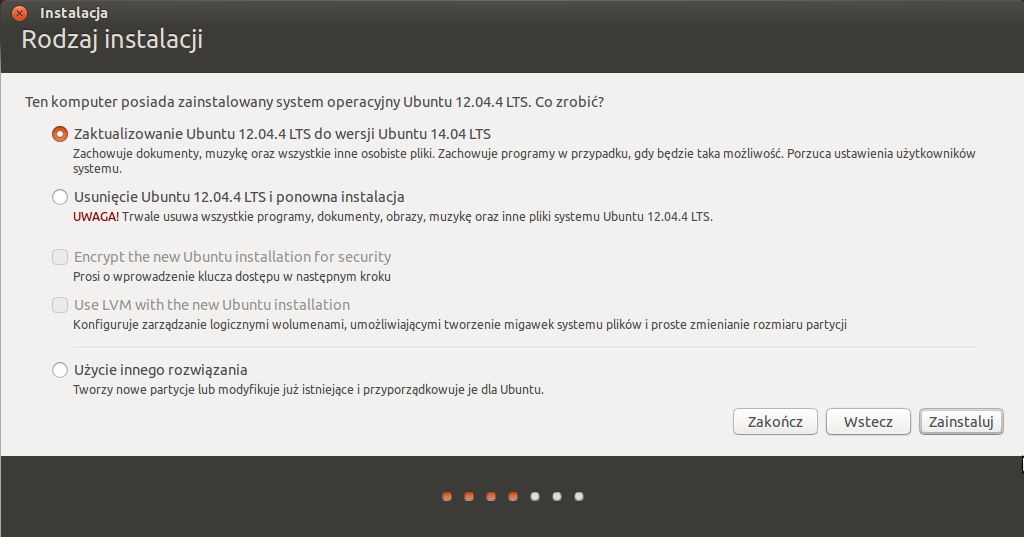
\includegraphics[scale=0.5]{images/instalator_partycjonowanie_obok_ubuntu.png}
\end{center}
Jeżeli instalator wykryje obecność wcześniej zainstalowanej innej wersji Ubuntu to zaproponuje kilka innych rozwiązań.

Po pierwsze zaproponuje aktualizację zainstalowanego systemu do najnowszego wydania. Wszystkie dane w katalogu domowym użytkownika zostaną zachowane: muzyka, filmy, dokumenty, pliki na pulpicie, osobieste ustaienia programów, zakładki i historia przeglądarki itp.
Skasowane zostaną zainstalowane w systemie programy oraz ustawienia systemowe. Instalator zaktualizuje istniejące na dysku oprogramowanie i ewentualnie pobierze aktualizacje z internetu (jeżeli wybrałeś wcześniej tą opcję).

Drugą opcją jest usunięcie zainstalowanego Ubuntu i ponowna instalacja systemu. Wszystkie dane zostaną wymazane.
\begin{flushright}
Kliknij na przycisk \textbf{Zainstaluj} aby przejść dalej.\\
Zostaniesz poproszony o potwierdzenie. Upewnij się, że wszystko jest w pożądku i kliknij \textbf{Naprzód}.\\
W tym momencie wybrane zmiany zostaną zapisane na dysku twardym.
\end{flushright}
\clearpage

\subsubsection{Instalacja obok Windowsa}
\begin{center}
	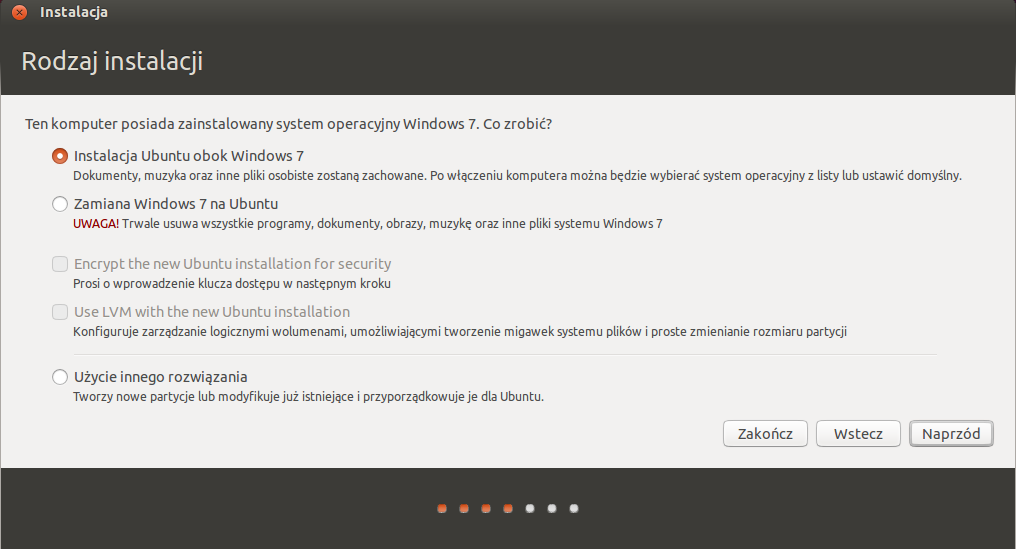
\includegraphics[scale=0.5]{images/instalator_partycjonowanie_obok_wondows7.png}
\end{center}
Jeżeli instalator wykryje obecnosć wcześniej zainstalowanego systemu Windows to zaproponuje inne rozwiązanie. Opcja "Zamiana Windows na Ubuntu" wymaże całą zawartość partycji Windows (wraz ze wszystkimi danymi) i zamiast tego zainstaluje Ubuntu. Zostało to opisane dwie strony wcześniej.
\begin{flushright}
Kliknij na przycisk \textbf{Zainstaluj} aby przejść dalej.
\end{flushright}
\clearpage
\begin{center}
	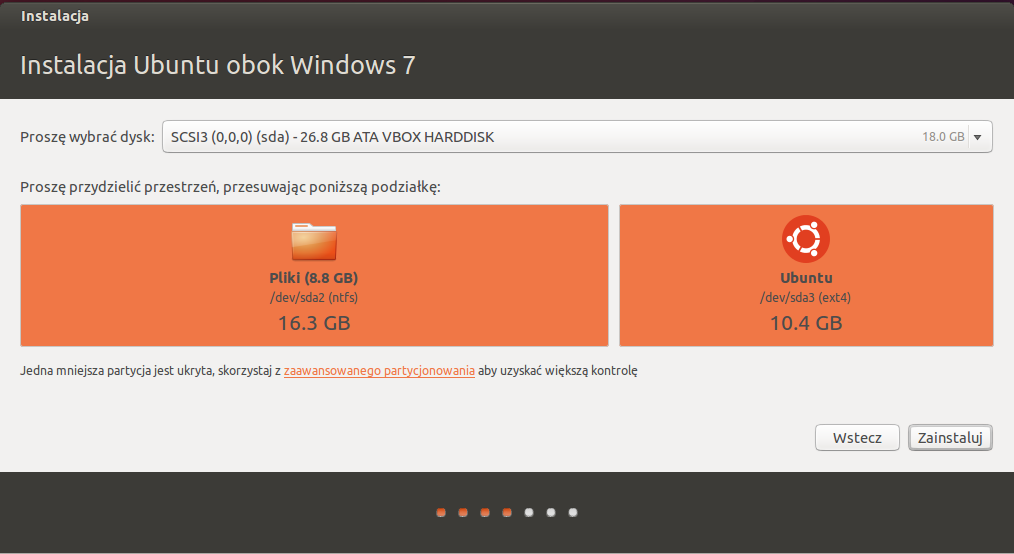
\includegraphics[scale=0.5]{images/instalator_partycjonowanie_obok_wondows7_2.png}
\end{center}
Drugą możliwością jest instalacja Ubuntu obok już zainstalowanego systemu Windows. Jeżeli wybierzesz tę opcję to następny ekran pozwoli wybrać o ile instalator ma zmniejszyć partycję na której zainstalowany jest system Windows. Użyj myszy aby przesunąć pomarańczową podziałkę w lewo (więcej miejsca dla Ubuntu) lub w prawo(więcej miejsca dla Windowsa). Oryginalna partycja systemu Windows jest oznaczona na tym obrazie jako "Pliki". Pamiętaj, że ubuntu potrzebuje minimum 6,2 gigabajta przestrzeni, ale tak mała partycja zostanie prawie w całości wypełniona przez system i na Twoje pliki pozostanie niewiele miejsca.

\begin{flushright}
Kliknij na przycisk \textbf{Zainstaluj} aby przejść dalej.\\
Zostaniesz poproszony o potwierdzenie. Upewnij się, że wszystko jest w pożądku i kliknij \textbf{Naprzód}.\\
W tym momencie wybrane zmiany zostaną zapisane na dysku twardym.
\end{flushright}
\clearpage

\subsubsection{Szyfrowanie dysku twardego}
\begin{center}
	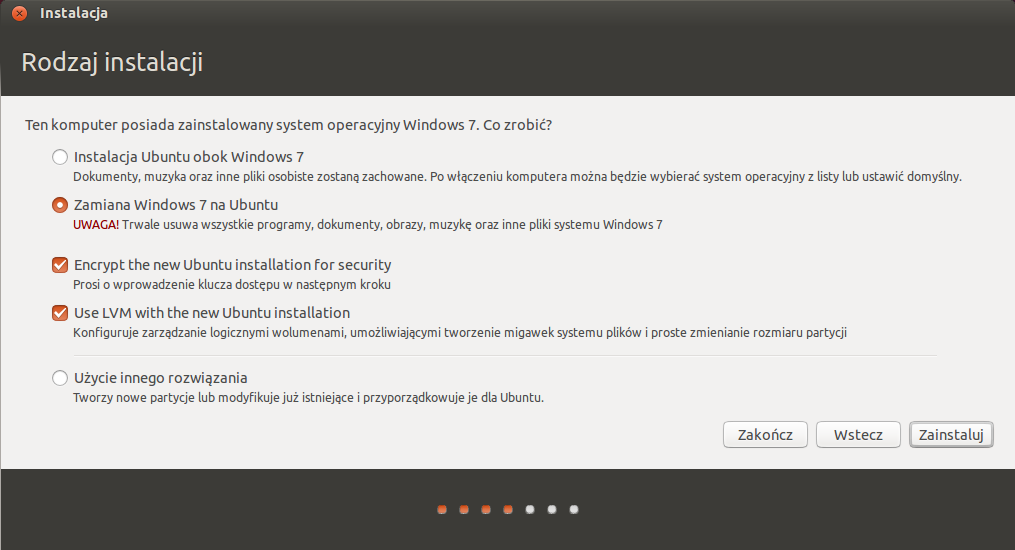
\includegraphics[scale=0.5]{images/instalator_partycjonowanie_szyfrowanie1.png}
\end{center}
Przy wyborze jednego z automatycznych rozwiązań partycjonowania miałeś możliwości zastosowania szyfrowania dysku twardego. Wybranie tej opcji ukaże ci okno jak na powyższym obrazku. Zaszyfrowanie dysku twardego sprawie, że nikt nie uzyska dostępu do twoich danych ani nie zmodyfikuje zainstalowanego systemu. Wadą tego rozwiązania jest pewien narzut na procesor komputera i związane z tym zmniejszenie płynności działania komputera. Nowoczesne procesory zapewniają akcelerację sprzętową dla obliczeń kryptograficznych, w związku z czym utrata wydajności będzie się mieścić w granicach 5\% przy intensywnych opracacjach dyskowych.
\begin{flushright}
Kliknij na przycisk \textbf{Zainstaluj} aby przejść dalej.
\end{flushright}
\clearpage
\begin{center}
	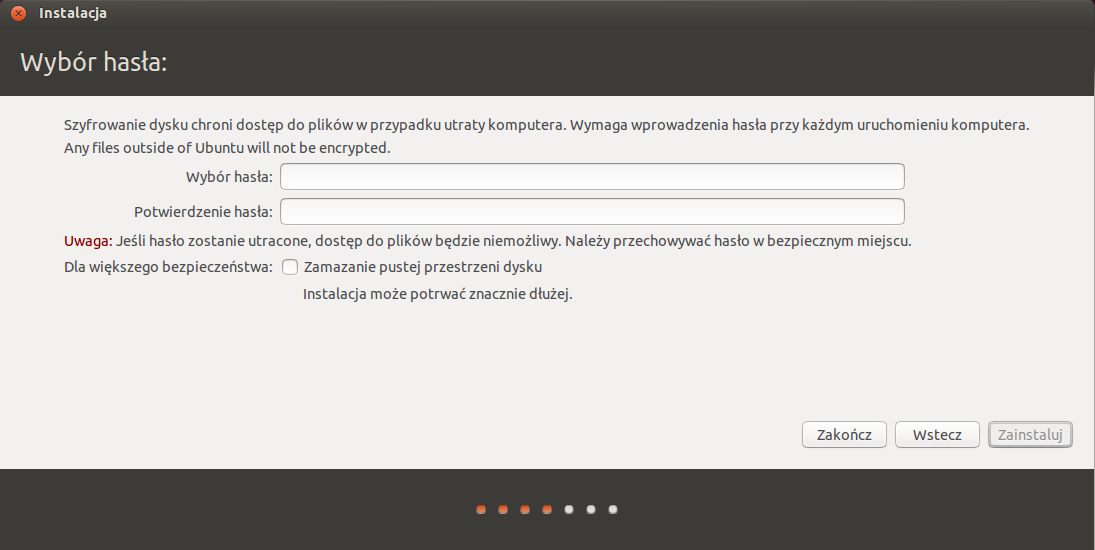
\includegraphics[scale=0.5]{images/instalator_partycjonowanie_szyfrowanie2.png}
\end{center}
Na tym ekranie podaj hasło - klucz do dysku twardego. To nie jest to samo hasło, które ustawisz dla swojego systemowego konta a jedynie hasło umożliwiające dostęp do danych zapisanych na dysku twardym. Pamiętaj, że jeżeli zapomnisz hasła jakie zostanie tu wprowadzone, nie będzie możliwości odzyskania zaszyfrowanych danych. Postaraj się też aby hasło nie było łatwe do odgadnięcia, ale łatwe dla ciebie do zapamiętania.

Opcja "Zamazanie pustej przestrzeni dysku" powoduje, że niewykorzystywana, wolna przestrzeń dysku zostanie nadpisana losowymi danymi. Taka operacja znacznie utródnia potencjalnym włamywaczą włamanie się do twoich danych. Miej na uwadze, że zamazywanie pustej przestrzeni może trwać bardzo długo, w zależności do tego ile miejsca przeznaczysz na Ubuntu.

\begin{flushright}
Kliknij na przycisk \textbf{Zainstaluj} aby przejść dalej.\\
Zostaniesz poproszony o potwierdzenie. Upewnij się, że wszystko jest w pożądku i kliknij \textbf{Naprzód}
W tym momencie wybrane zmiany zostaną zapisane na dysku twardym.\\
\end{flushright}
\clearpage

\subsection{Zaawansowane partycjonowanie}
\begin{center}
	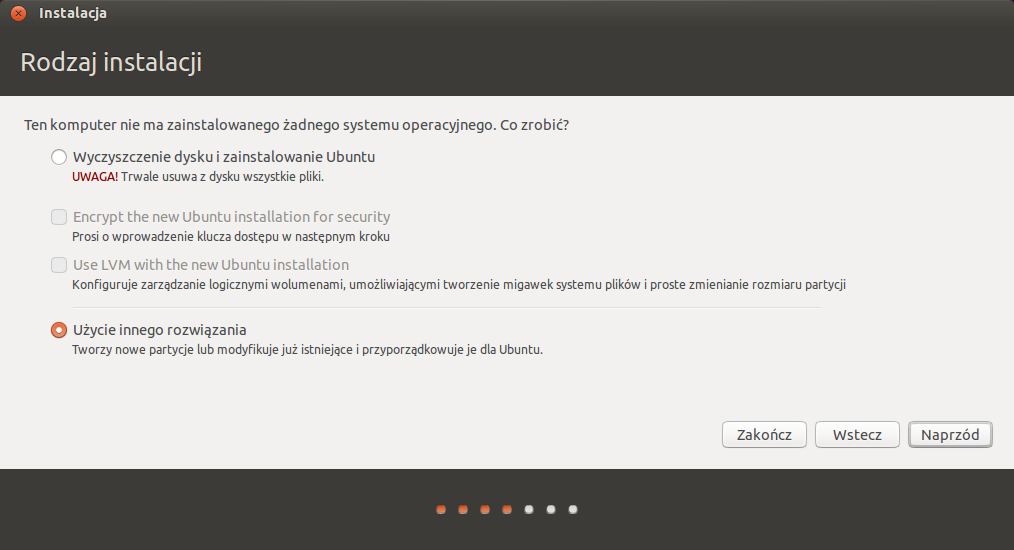
\includegraphics[scale=0.5]{images/instalator_partycjonowanie_gparted1.png}
\end{center}
"Użycie innego rozwiązania" uruchamia program GParted, który umożliwia nieograniczone modyfikowanie partycji na dysku twardym. Jest to opcja dla bardziej zaawansowanych użytkowników, którzy mają świadomość tego jak działa partycjonowanie i jak powinien zostac podzielony ich dysk twardy. Jednak jeżeli na swoim komputerze maasz zainstalowany więcej niż jeden system operacyjny lub z jakiegoś innego powodu przedstawione wcześniej opcje nie spełniają twoich wymagań, to konieczne będzie sięgnięcie do zaawansowanego partycjonowania.

Do GParted warto zajrzeć jeszcze z jednego powodu. Podział partycji stosowany przez automatyczną instalację nie jest idealny. Ręczne ustawienie partycji da większa kontrolę i pozwoli znacznie lepiej dopasować układ partycji.
\begin{flushright}
Kliknij na przycisk \textbf{Naprzód} aby przejść dalej.
\end{flushright}
\clearpage

\subsubsection{Główne okno programu GParted}
\begin{center}
	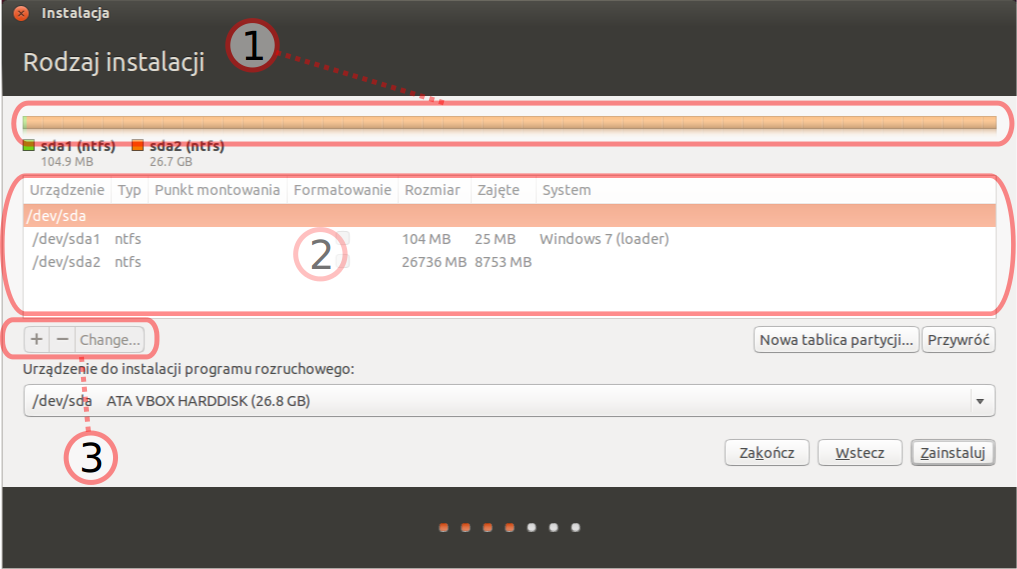
\includegraphics[scale=0.5]{images/instalator_partycjonowanie_gparted2.png}
\end{center}
Na powyższym obrazku widzisz głowne okno programu GParted. Wykryty został układ partycji na dysku twardym. Poziomy pasek (1) rozciągający się na całą szerokość okna jest graficzną reprezentacją układu partycji. Poniżej paska znajduje się legenda objaśnijaca użyte kolory. Tabela (2) znajdująca się w centralnej części okna przedstawia szczegółowe informacje na temat partycji na dysku twardym. Zestaw przycisków (3) służy do dodawania partycji(+), usówania partycji (-) lub ich modyfikacji(Change). Na chwilę obecną inne rzeczy nas nie interesują.

Powyższy układ dysków twardych oraz partycji jest tylko przykładem skonstruowanym na maszynie wirtualnej. Na Twoim komputerze liczby będą inne.

\clearpage
\begin{center}
	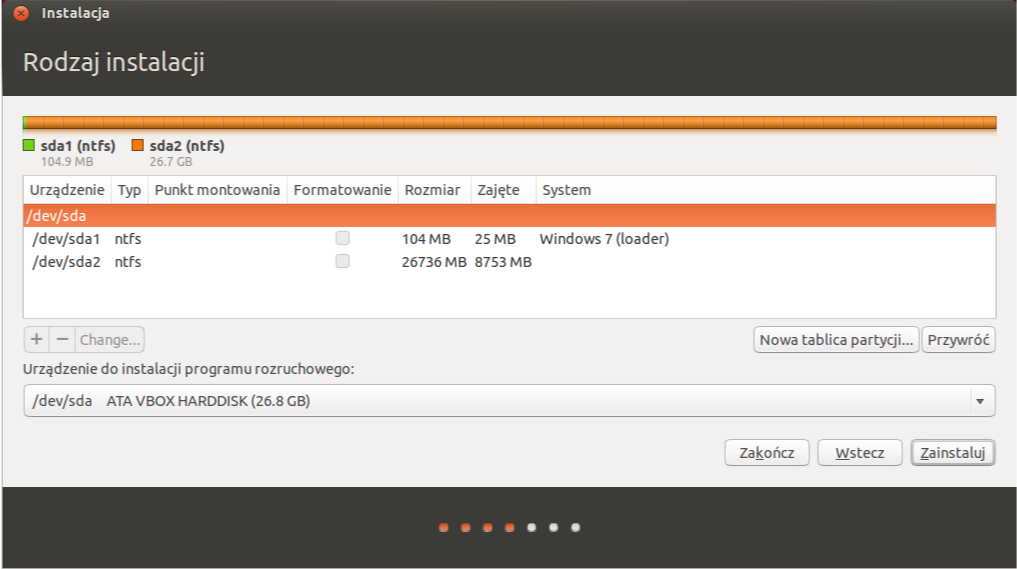
\includegraphics[scale=0.5]{images/instalator_partycjonowanie_gparted2_czysty.png}
\end{center}
Tabela umieszczona w centrum tego okna przedstawia informacje o poszczególnych partycjach obecnych na dysku twardym. Objaśnienie poszczególnych kolumn:
\begin{description}
\item[Urzadzenie] - Ścierzka do poszczególnych partycji na dysku twardym. Są to oznaczenia stosowane w systemach Unikoswych, do których należy Linux a więc i Ubuntu i opisują jak rozpoznawane są poszczególne partycje. W tym wypadku:
	\begin{description}
	\item[/dev/] - skrót od "Device", urządzenie
	\item[sda] - oznaczenie pierwszego dysktu twardego.
		\begin{description}
			\item[sd] - dysk na złączu SATA (sata disc)
			\item[a] - pierwszy dysk. Drugi dysk twardy miałby literę "b", trzeci "c" i tak dalej.
		\end{description}
	\item[sda1] - pierwsza partycja na pierwszym dysku twardym.
	\item[sda2] - druga partycja na pierwszym dysku twardym.
	\end{description}
\item[Typ] - rodzaj systemu plików. Sposób w jaki partycja została sformatowana. System Windows korzysta z ntfs, Ubuntu może korzystać z różnych.
\item[Punkt montowania] - miejsce w którym dana partycja zostanie "zamontowana", katalog w którym będzie widoczna zawartość tej partycji.
\item[Formatowanie] - zaznaczając to pole informujesz instalator, że dana partycja ma zostać sformatowana. Oznacza to utratę wszystkich danych na niej zapisanych.
\item[rozmiar] - pojemność partycji w megabajtach.
\item[Zajęte] - ile miejsca zostało zajęte na tej partycji
\item[System] - system operacyjny zainstalowany na danej partycji. Nie zawsze da się rozpoznać zainstalowany system. Nie każda partycja musi mieć zainstalowany system operacyjny. 
\end{description}
\clearpage
\subsubsection{Zaawansowane partycjonowanie - Instalacja obok systemu Windows}
\begin{center}
	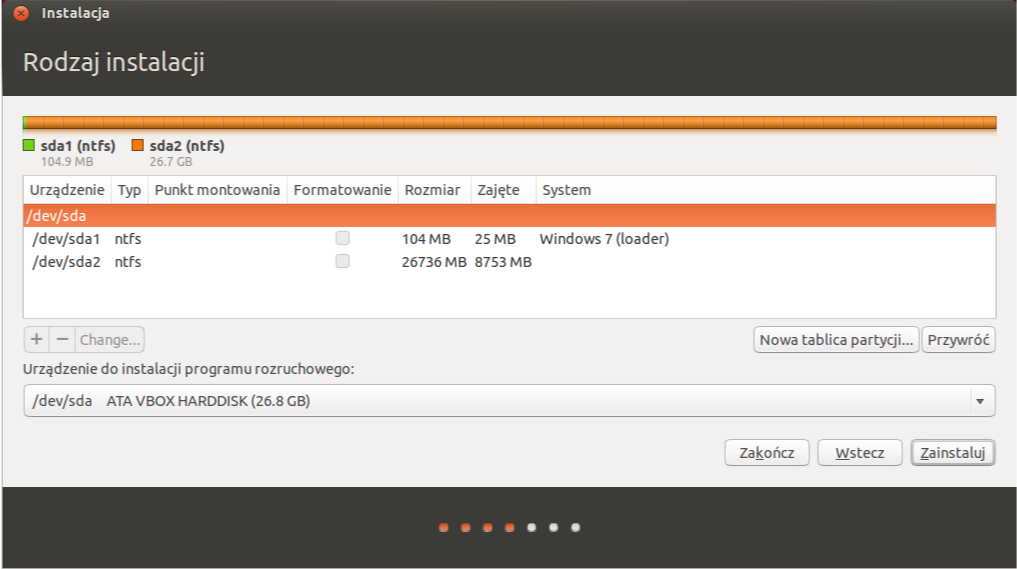
\includegraphics[scale=0.5]{images/instalator_partycjonowanie_gparted2_czysty.png}
\end{center}

Na powyższym obrazku widać dwie partycje utworzone przez instalator systemu Windows7. Partycja zielona o rozmiarze 104 megabajtów służy jako partycja dla programu rozruchowego systemu Windows. Duża, pomarańczowa partycja (26736 megabajtów) jest główna partycją systemu Windows7. Bardzo podobny układ partycji stosowany jest przez każdy z systemów z rodziny Windows.

Pierwszym krokiem jest zrobienie miejsca dla systemu Ubuntu. Kliknij na partycję /dev/sda2. Następnie kliknij na przycisk "Change" znajdujący się pod tabelą.. W otwartym oknie możesz zmniejszyć rozmiar wybranej partycji.
\clearpage

\begin{wrapfigure}{R}{0.4\textwidth}
		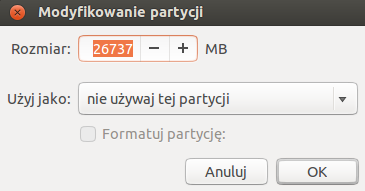
\includegraphics[scale=1]{images/instalator_partycjonowanie_gparted_zmniejszenie_partycji_windows.png}
\end{wrapfigure}
W polu Rozmiar podaj nowy rozmiar partycji. O tym ile miejsca potrzebujesz na Ubuntu przeczytasz w rozdziale \ref{subsubsec:ile_miejsca}: Ile miejsca przeznaczyć na Ubuntu. W polu podajesz rozmiar partycji w megabajtach. Jeden gigabajt to 1024 megabajty.\\
Upewnij się, że wybrano opcję "nie używaj tej partycji". Teraz kliknij przycisk \textbf{OK} a następnie \textbf{Naprzód} aby dokonać zmiany na partycji. Wykonanie żądanej zmiany może trwać dłuższą chwilę.

Na schemacie pojawiła się pusta, "dostępna przestrzeń" oznaczona kolorem szarym. Kliknij a nią, a następnie na przycisk (+) aby stworzyć nową partycję.
\begin{center}
	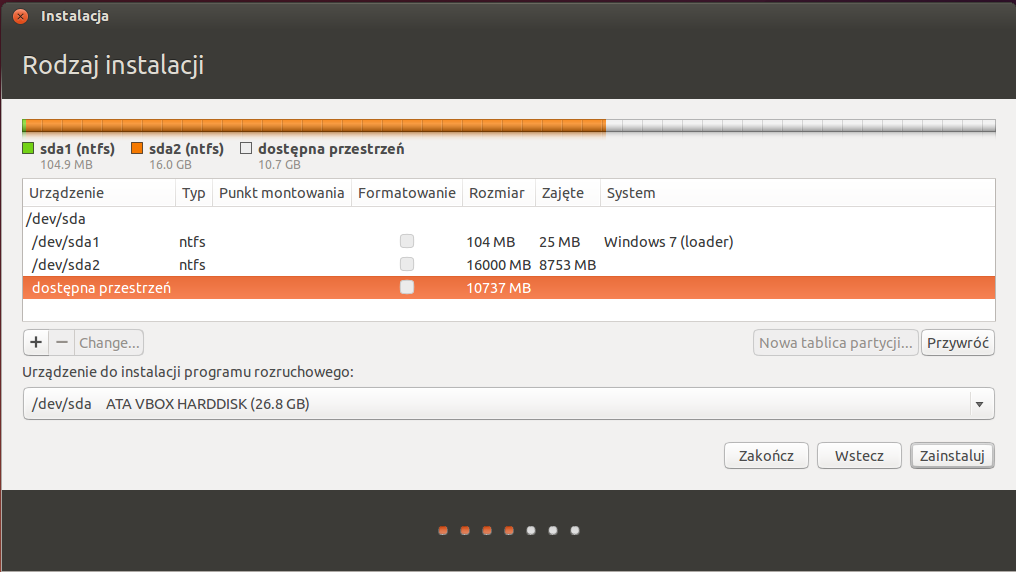
\includegraphics[scale=0.7]{images/instalator_partycjonowanie_gparted3.png}
\end{center}
\clearpage

\begin{wrapfigure}{R}{0.4\textwidth}
		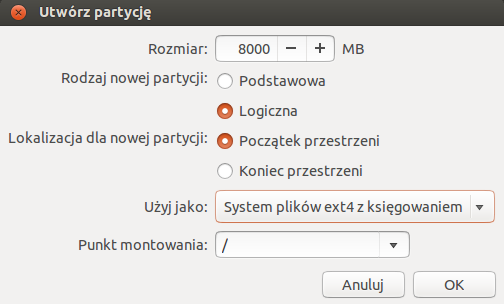
\includegraphics[scale=0.8]{images/instalator_partycjonowanie_gparted_dodaj_root.png}
\end{wrapfigure}
Po pierwsze musimy stworzyć partycję podstawową dla Ubuntu. O ilości miejsca potrzebnej na poszczególne partycje przeczytasz w sekcji \ref{subsubsec:ile_miejsca}: "Ile miejsca przeznaczyć na Ubuntu". Pozostałe opcje ustaw jak na rysunku.
\begin{description}
\item[Rozmiar] - rozmiar partycji w megabajtach
\item[Rodzaj nowej partycji] - jako, że system Windows korzysta z tablicy partycji ms-dos to jesteśmy ograniczeni do 4 partycji podstawowych. Aby nie było problemu, dla Ubuntu utworzymy partycje logiczne.
\item[Lokalizacja dla nowej partycji] - Czy partycja zostanie wyrównana do poczatku wolnej przestrzeni czy do jej końca. Nie ma to znaczenia dla działania systemu.
\item[Użyj jako] - jaki system plików ma być użyty do sformatowania tej partycji. Do wyboru jest wiele, ale w ramach tego przewodnika korzystamy z systemu ext4 z księgowaniem\footnote{Tematyka różnych systemów plików jest bardzo rozległa i z łatwością wypełniłaby kolejny Przewodnik.}
\item[Punkt montowania] - to nasza główna partycja, więc musi się znaleźdź na początku\footnote{W systemach Windows drzewo katalogów "zaczyna się" na "C:\textbackslash\textbackslash". W systemach Linuksowych zaczyna się na "/"}.
\end{description}
Kliknij na przycisk \textbf{OK} aby utworzyć nową partycję.
\clearpage
\begin{wrapfigure}{R}{0.4\textwidth}
		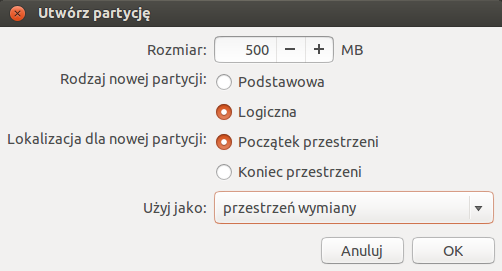
\includegraphics[scale=0.8]{images/instalator_partycjonowanie_gparted_dodaj_swap.png}
\end{wrapfigure}
Teraz utwórz partycję wymiany. Więcej o tej partycji przeczytasz w w sekcji \ref{subsubsec:ile_miejsca}: "Ile miejsca przeznaczyć na Ubuntu". Pozostałe opcje ustaw jak na rysunku. Kliknij na przycisk \textbf{OK} aby utworzyć nową partycję.

\begin{wrapfigure}{L}{0.4\textwidth}
		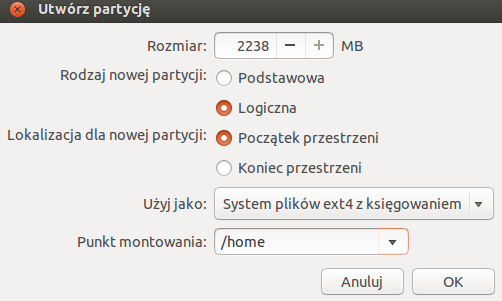
\includegraphics[scale=0.8]{images/instalator_partycjonowanie_gparted_dodaj_home.png}
\end{wrapfigure}
Na koniec pozostało utworzenie partycji domowej. Więcej o tej partycji przeczytasz w w sekcji \ref{subsubsec:ile_miejsca}: "Ile miejsca przeznaczyć na Ubuntu". Pozostałe opcje ustaw jak na rysunku. Kliknij na przycisk \textbf{OK} aby utworzyć nową partycję.
\clearpage

\begin{center}
	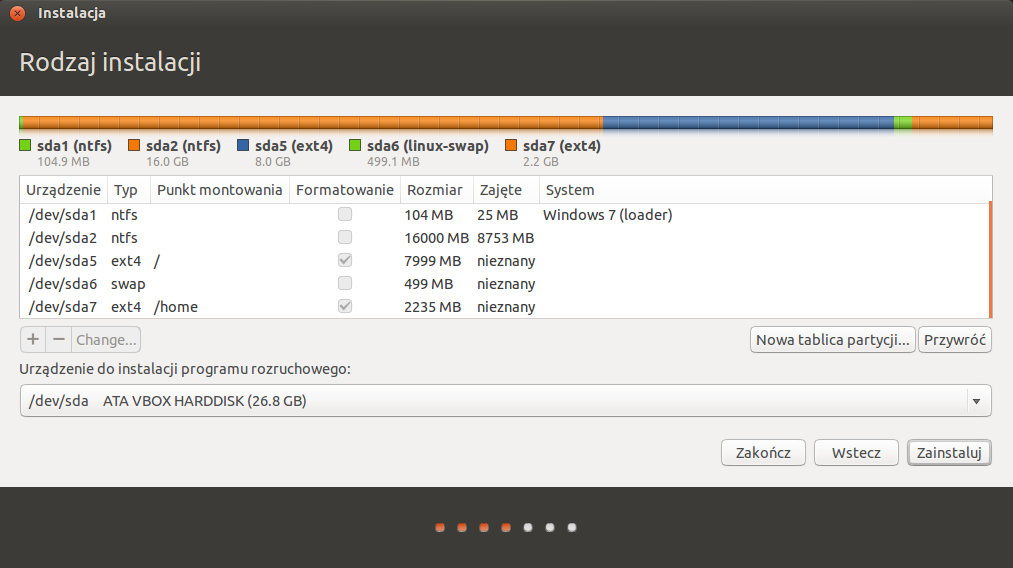
\includegraphics[scale=0.7]{images/instalator_partycjonowanie_gparted4.png}
\end{center}
Ekran programu GParted wygląda teraz mniej więcej tak jak na rysunku powyżej. Masz dwie partycje systemu Windows (ntfs), partycję wymiany systemu Linux (swap) oraz dwie partycje dla systemu Ubuntu (ext4). Upewnij się, że partycje ntfs \textbf{nie} są zaznaczone do sformatowania, zaś partycje ext4 tak. Kliknij na przycisk \textbf{Naprzód} aby wprowadzić zmiany na partycjach. Teraz możesz powrócić do lektury procesu instalacji w miejscu gdzie go przerwałeś.\\
Powrót do \ref{subsub:instalator_strefa_czasowa}: Wybór sterfy czasowej.
\clearpage
	\subsection{Rozwiązywanie problemów z instalacją}
\section{Pierwsze uruchomienie systemu}
	\subsection{Rzeczy do zrobienia po instalacji Ubuntu}
	\label{sec:rzeczy_do_zrobienia_po_instalacji}
\section{Pulpit Ubuntu Unity}

%rozwiązywanie problemów z Windows 8
\end{document}
